% Created 2018-03-31 Sat 07:38
% Intended LaTeX compiler: xelatex
\documentclass[presentation]{beamer}
\usepackage{graphicx}
\usepackage{grffile}
\usepackage{longtable}
\usepackage{wrapfig}
\usepackage{rotating}
\usepackage[normalem]{ulem}
\usepackage{amsmath}
\usepackage{textcomp}
\usepackage{amssymb}
\usepackage{capt-of}
\usepackage{hyperref}
\usepackage{circuitikz}
\usetheme[titleformat=smallcaps,progressbar=frametitle]{metropolis}
\author{Moritz Kütt (kuett@princeton.edu)}
\date{March 14, 2018}
\title{How can Germany become a Member of the Ban Treaty}
\title[Germany joins the Ban Treaty]{How can Germany become a \\Member of the Ban Treaty}
\author[M. Kütt]{Moritz Kütt (kuett@princeton.edu)}
\institute{Program on Science and Global Security \\[2em] \vfill \ccbysa \\[0.4em] \tiny \textcolor{gray!85}{Detailed image references at the end of the presentation.}}
\usepackage{orgbeamerdefaults}
\setbeamerfont{block title}{size=\footnotesize}
\setbeamerfont{block title alerted}{size=\footnotesize}
\setbeamerfont{block title example}{size=\footnotesize}
\setbeamerfont{block body}{size=\scriptsize}
\setbeamerfont{block body alerted}{size=\scriptsize}
\setbeamerfont{block body example}{size=\scriptsize}
\usepackage[none]{hyphenat}
\definecolor{nuco}{HTML}{e2f2fa}
\setsansfont[ItalicFont={Fira Sans Condensed Italic},BoldFont={Fira Sans Medium},BoldItalicFont={Fira Sans Medium Italic}]{Fira Sans Condensed}
\hypersetup{
 pdfauthor={Moritz Kütt (kuett@princeton.edu)},
 pdftitle={How can Germany become a Member of the Ban Treaty},
 pdfkeywords={},
 pdfsubject={},
 pdfcreator={Emacs 25.3.1 (Org mode 9.1.2)}, 
 pdflang={English}}
\begin{document}

\maketitle

\begin{frame}[label={sec:org2829168}]{Outline}
\begin{enumerate}
\item Germany: A NU Perspective
\item More on Tactical Nuclear Weapons
\item (Domestic) Politics
\item Joining the Ban Treaty
\item Verification Options
\item Conclusion / Recommendations
\end{enumerate}

\note{
Assume TPNW is Ban Treaty
Some General Background
I'm not the expert on all things
Field of experst on tactical nuclear weapons and especially NATO
}
\end{frame}


\section{Germany: a NU Perspective}
\label{sec:org3a7e52d}
{
\usebackgroundtemplate{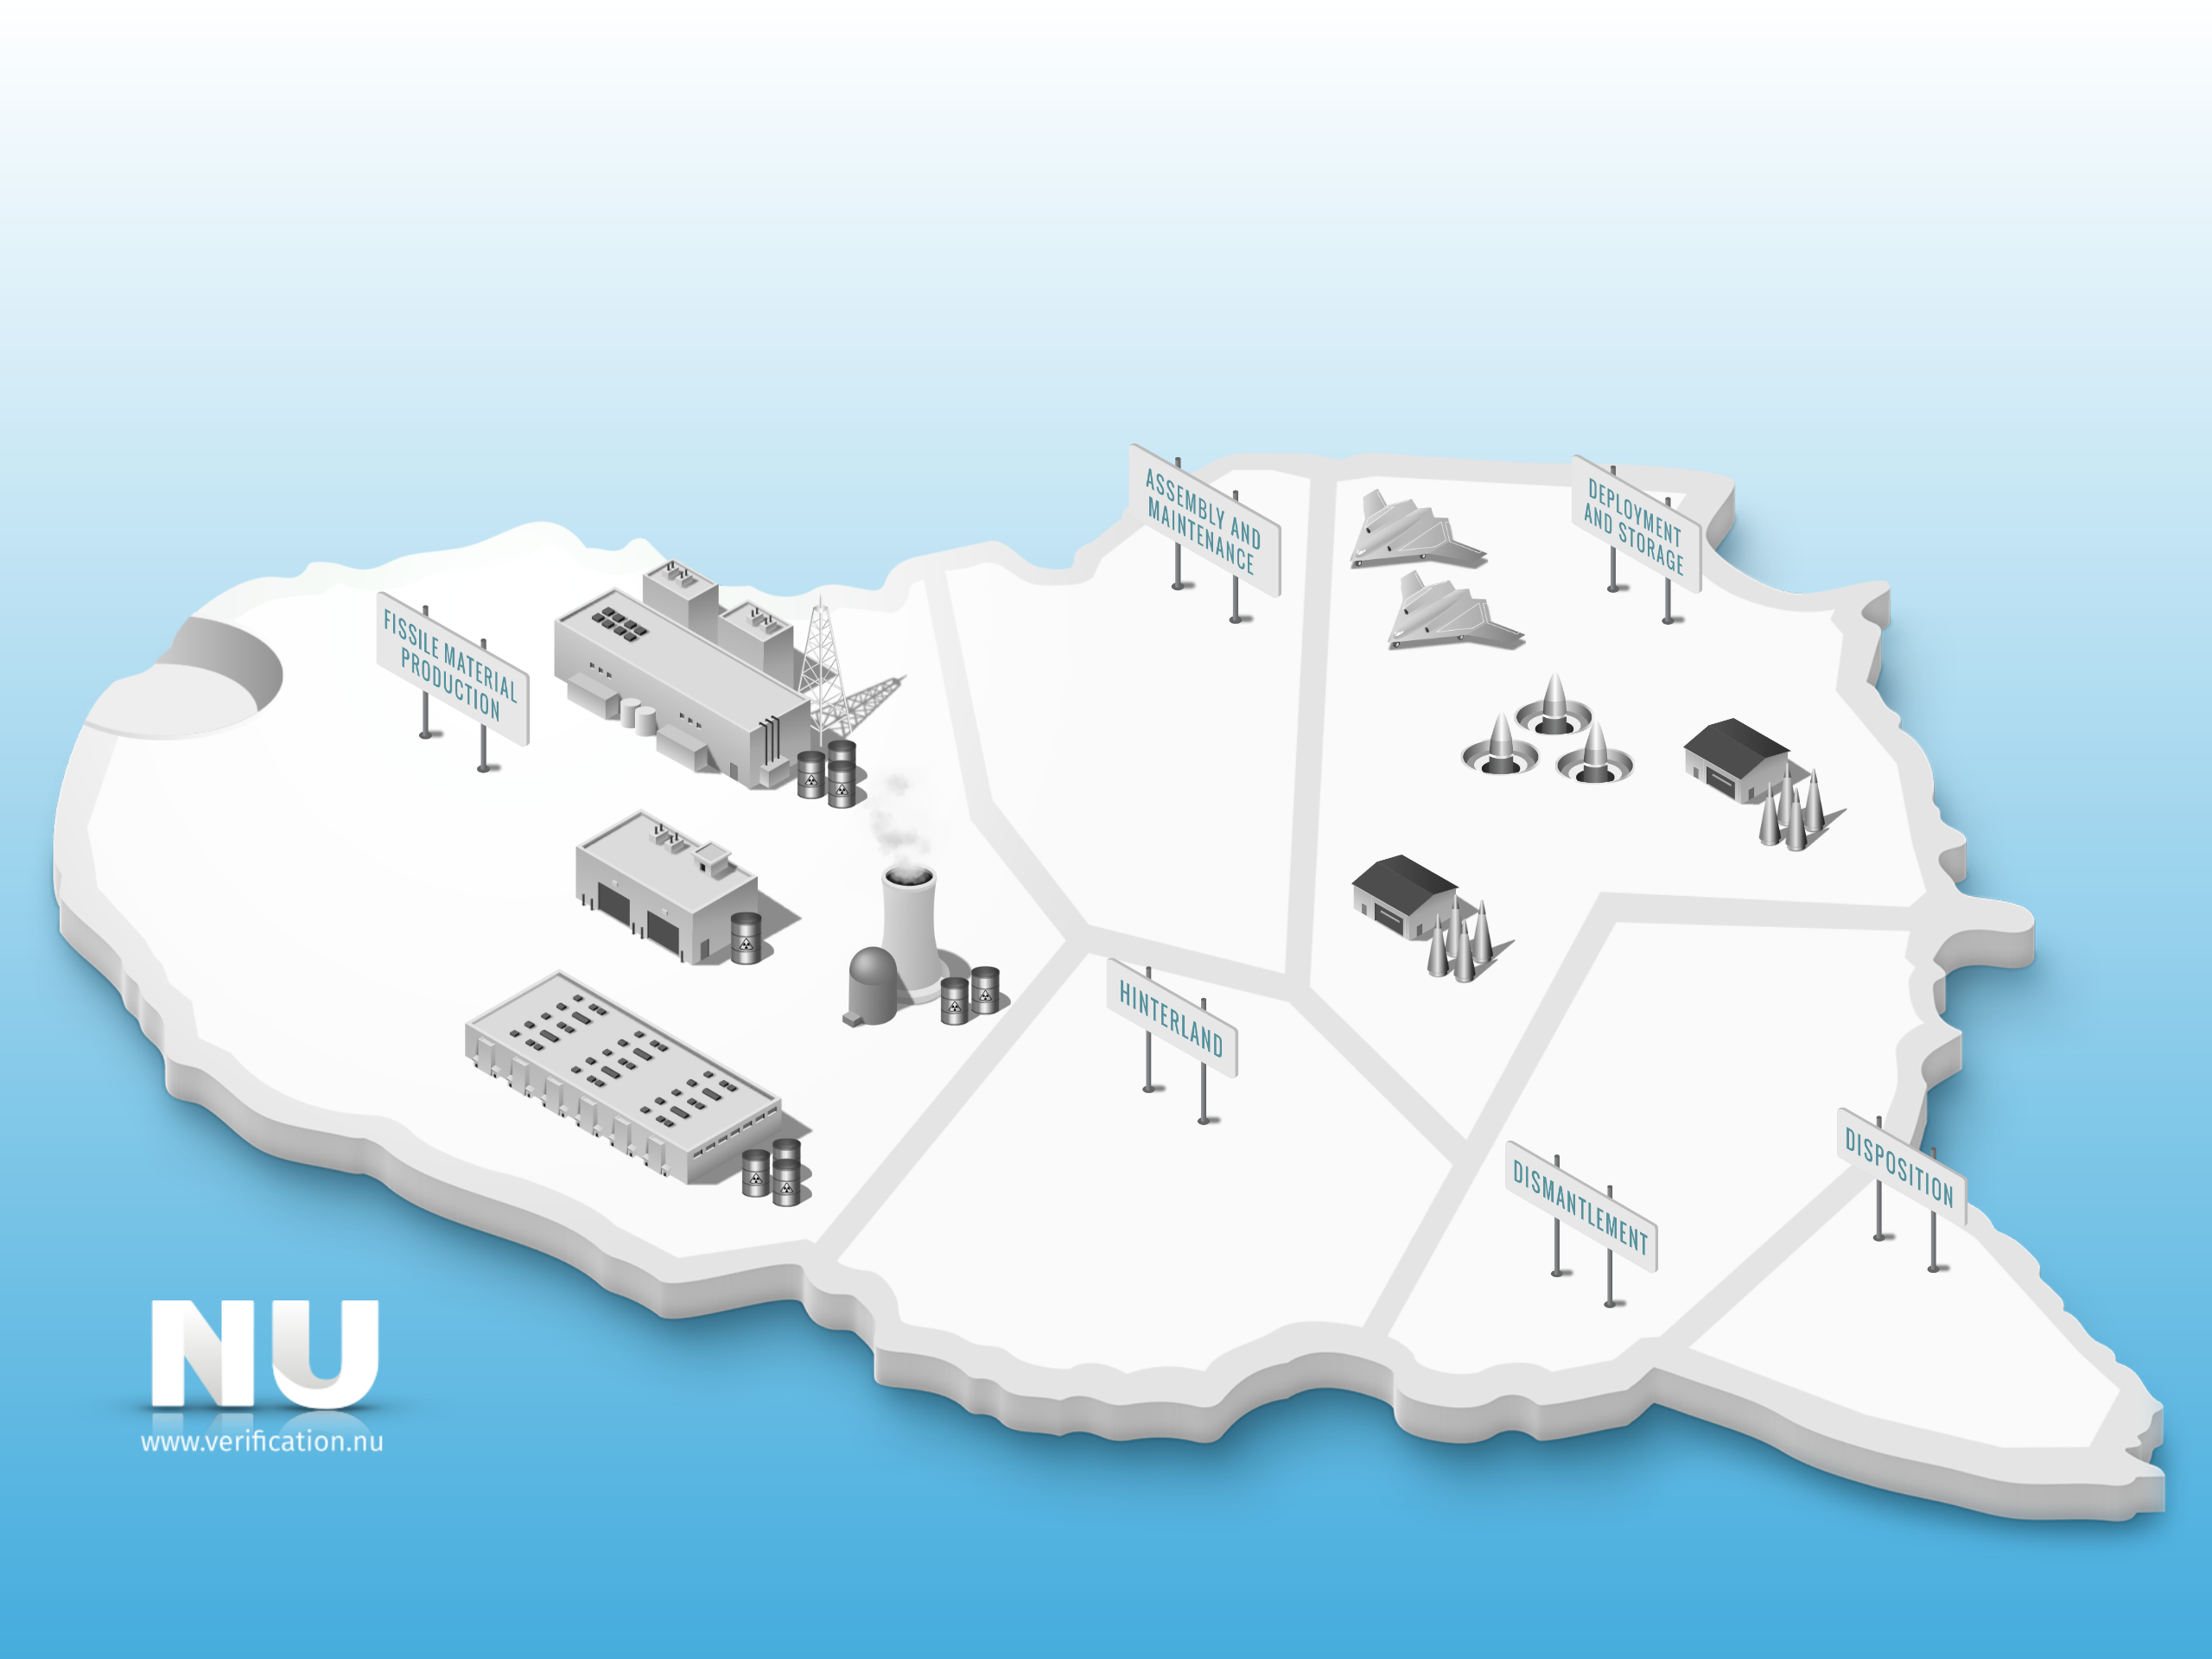
\includegraphics[width=\paperwidth]{localimages/cc/nu/germany/germany-full.png}}
\begin{frame}{Germany in Cold War Times}
\begin{tikzpicture}[remember picture,overlay]
    \tikzset{cout/.style={
        rounded corners = 0.04cm,
        draw,
        text width=2.5cm,
        align=flush left,
        rectangle callout,
        fill=nuco,
        font=\scriptsize}};
  
  \node [cout, callout absolute pointer={(2.4,0.4)}, anchor=north] at (0.6,3.8) {
  \alert{Fuel Fabrication} \\ \usebeamercolor[fg]{normal text}
  \tiny
  Framatome operates a plant in Lingen with a capacity of 650tHM/y\\
  };
  \node [cout, callout absolute pointer={(2.2,-1.6)},anchor=north] at (0.6,-2.3) {\alert{Uranium Enrichment} \\ \usebeamercolor[fg]{normal text}
  \tiny
  URENCO operates a plant in Gronau with a capacity of 4,000 tSWU/a\\
};
  \node<1-> [cout, callout absolute pointer={(4.4,-1)}, anchor=north] at (3.7,-2.3) {
  \alert{Reactors} \\ \usebeamercolor[fg]{normal text}
  \tiny
  7 power reactors remain in operation, phase out planned\\
  8 research reactors};

  \node<1-> [cout, callout absolute pointer={(3.2, 1.8)}, anchor=north] at (3.7,3.8) {
  \alert{Reprocessing} \\ \usebeamercolor[fg]{normal text}
  \tiny
  Pilot plant in Karlsruhe, shutdown 1991 (35 tHM/y),\\ 
  Large plant in Wackersdorf cancelled (350 tHM/y)\\};

  \node<2-> [cout, rectangle, anchor=north] at (0.6,0.6) {
  \alert{Mining / Conversion} \\ \usebeamercolor[fg]{normal text}
  \tiny
  (West) Germany never had significant mining/conversion capacities\\};

  \node<2-> [cout, text width=5.5cm, callout absolute pointer={(8.5, 0.2)}, anchor=north] at (8.3,-2.3) {
  \begin{tcolorbox}[standard jigsaw, height=1.4cm, valign=top, width=\textwidth, sharp corners, size=tight, frame empty, opacityback=0]
  \alert{Tactical Nuclear Weapons} \\ \usebeamercolor[fg]{normal text}
  \tiny
  About 4000 nuclear weapons at approx. 200 different locations:\\
  \only<3->{Lance Missile}\only<3->{, Sergeant Missile}\only<3->{, Pershing I}%
  \only<4->{, Atomic Demolition Munitoin}\only<4->{, Artillery Shells}\only<4->{, Honest John Missile}%
  \only<5->{, Nike Anti Aircraft Missile}\only<5->{, Gravity Bombs}\only<5->{, Pershing II, ...}
  \end{tcolorbox}
};

  \tikzset{timage/.style={anchor=north west, inner sep=0pt}};
  \node<3-> [timage] at (-0.8, 3.8) {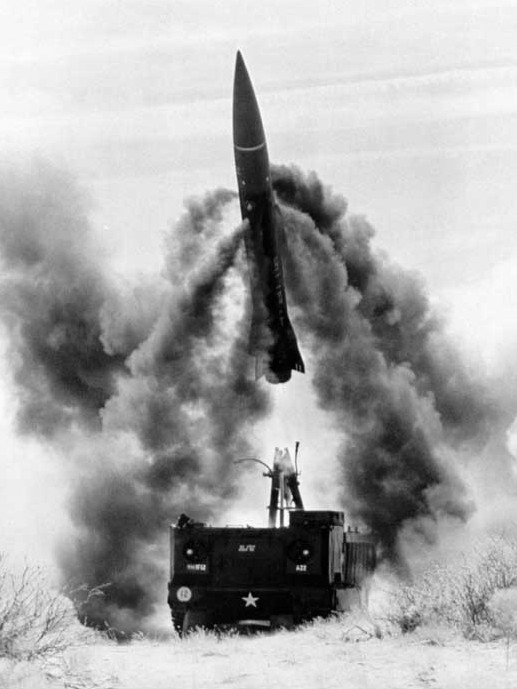
\includegraphics[width=2cm]{localimages/cc/weapons/MGM-52_Lance_02_ratio3-4.jpg}};
  \node<3-> [timage] at (1.2, 3.8) {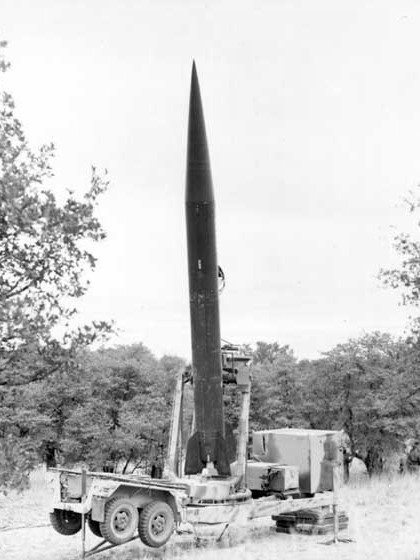
\includegraphics[width=2cm]{localimages/cc/weapons/MGM-29_Sergeant_05_ratio3-4.jpg}};
  \node<3-> [timage] at (3.2, 3.8) {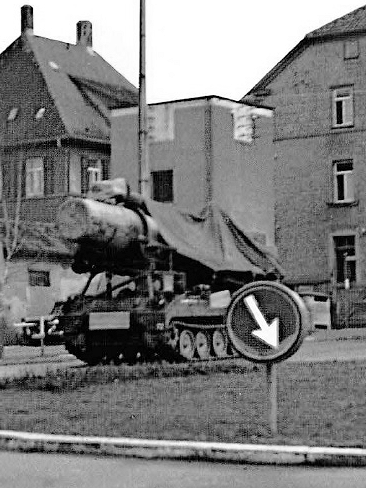
\includegraphics[width=2cm]{localimages/cc/weapons/OR_10.596B_13_ratio3-4.png}};

  \node<4-> [timage] at (-0.8, 1.13 ) {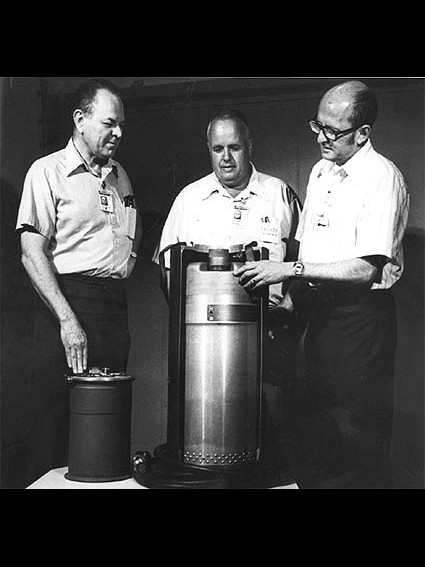
\includegraphics[width=2cm]{images/cc/weapons/Medium_Atomic_Demolition_Munition_(with_scientists)_ratio3-4.jpg}};
  \node<4-> [timage] at (1.2, 1.13) {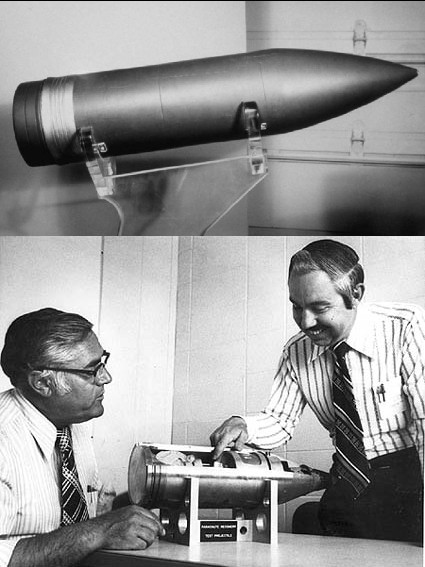
\includegraphics[width=2cm]{localimages/cc/weapons/Mk33-and-W48_ratio3-4.jpg}};
  \node<4-> [timage] at (3.2, 1.13) {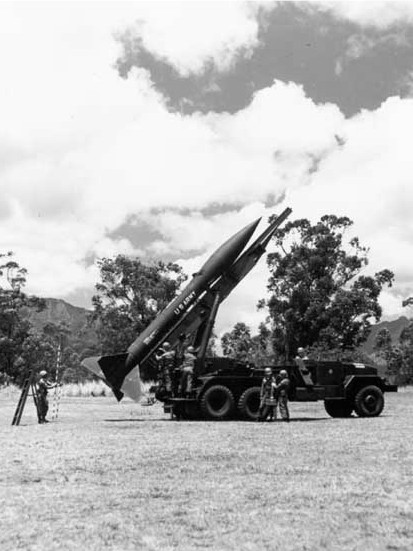
\includegraphics[width=2cm]{localimages/cc/weapons/MGR-1_Honest_John_06_ratio3-4.jpg}};

  \node<5-> [timage] at (-0.8, -1.54) {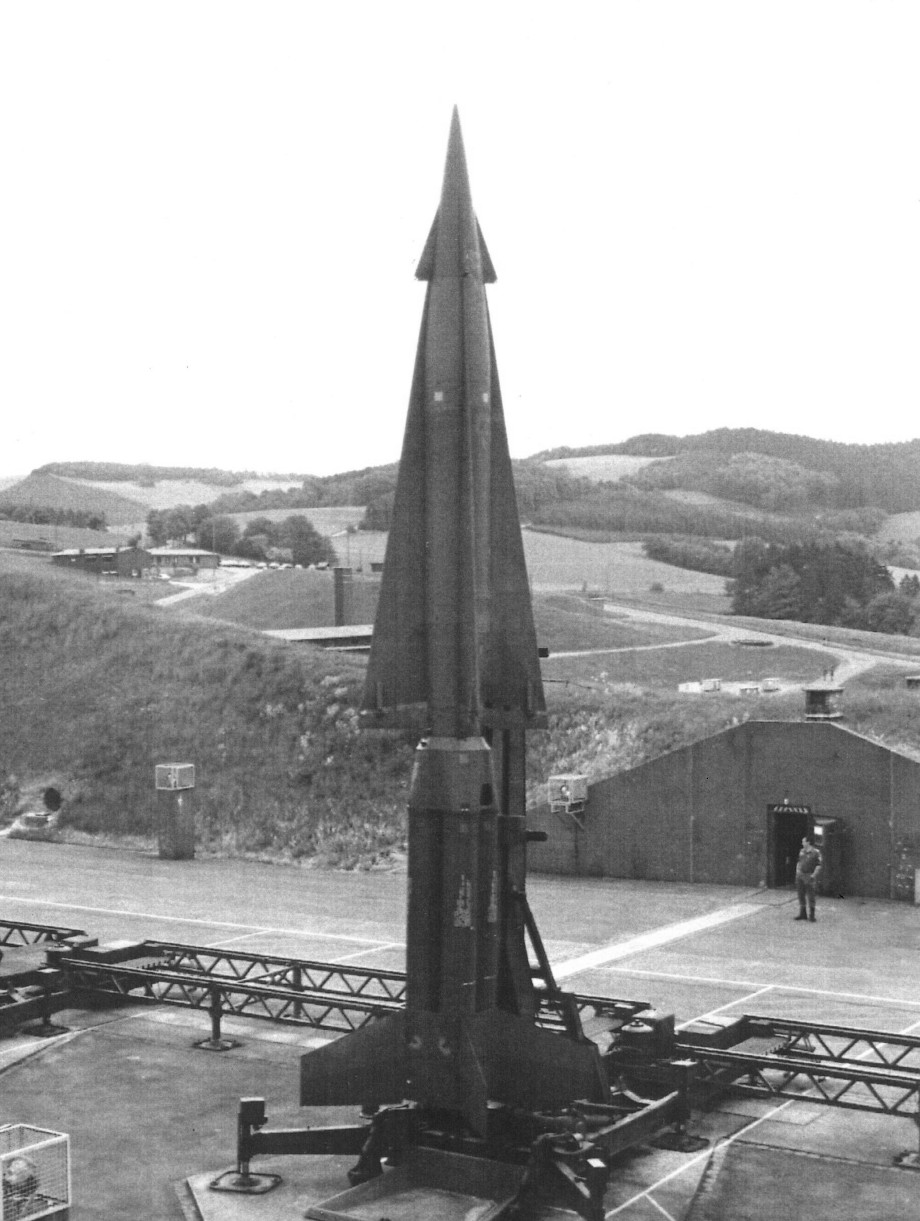
\includegraphics[width=2cm]{localimages/cc/weapons/Nike_Hercules_1980_ratio3-4.jpg}};
  \node<5-> [timage] at (1.2, -1.54) {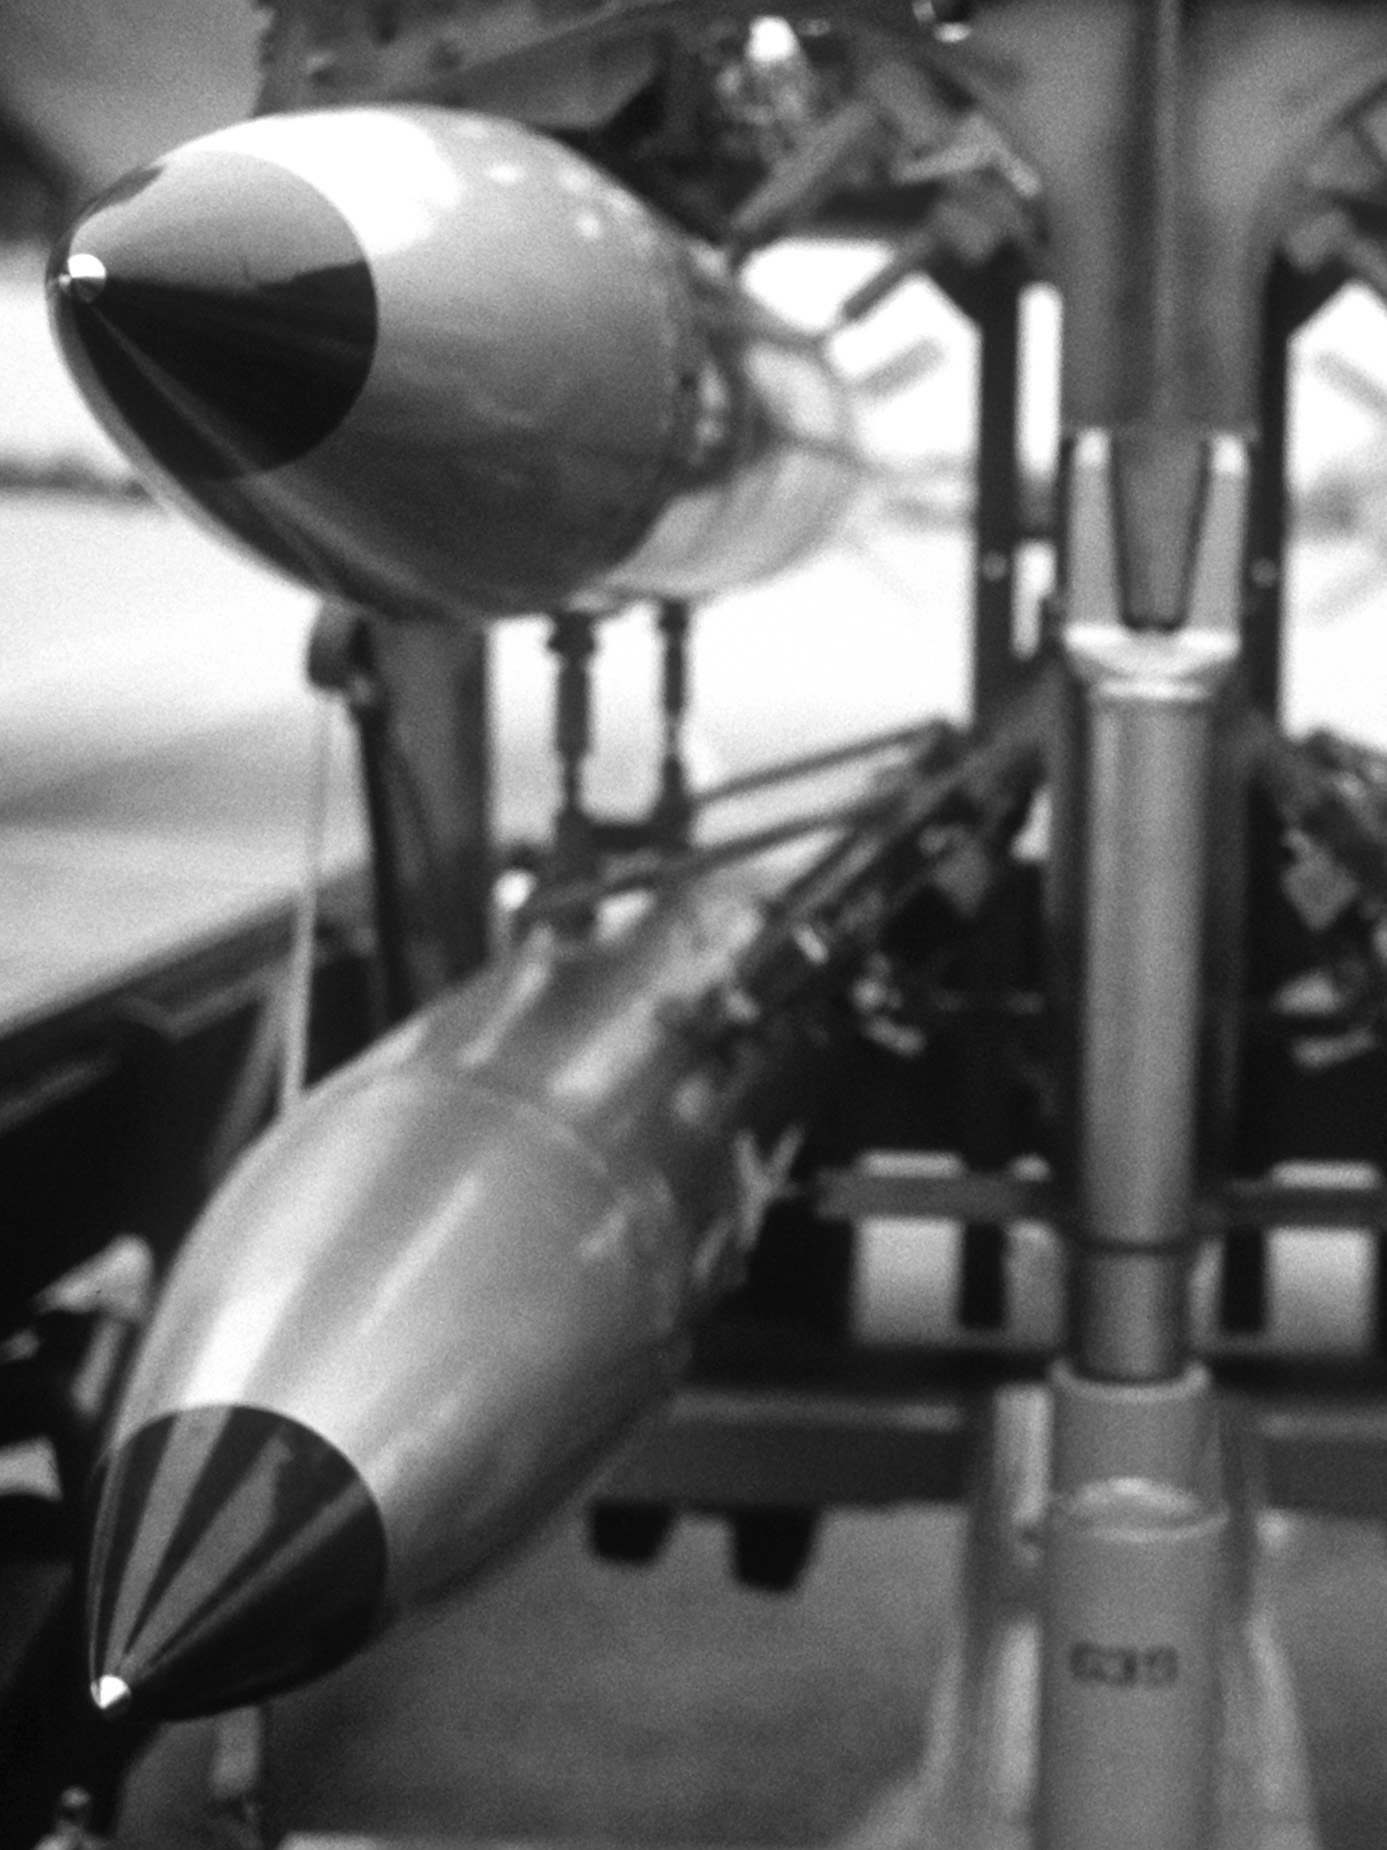
\includegraphics[width=2cm]{localimages/cc/weapons/B-61_bomb_rack_ratio3-4.jpg}};
  \node<5-> [timage] at (3.2, -1.54) {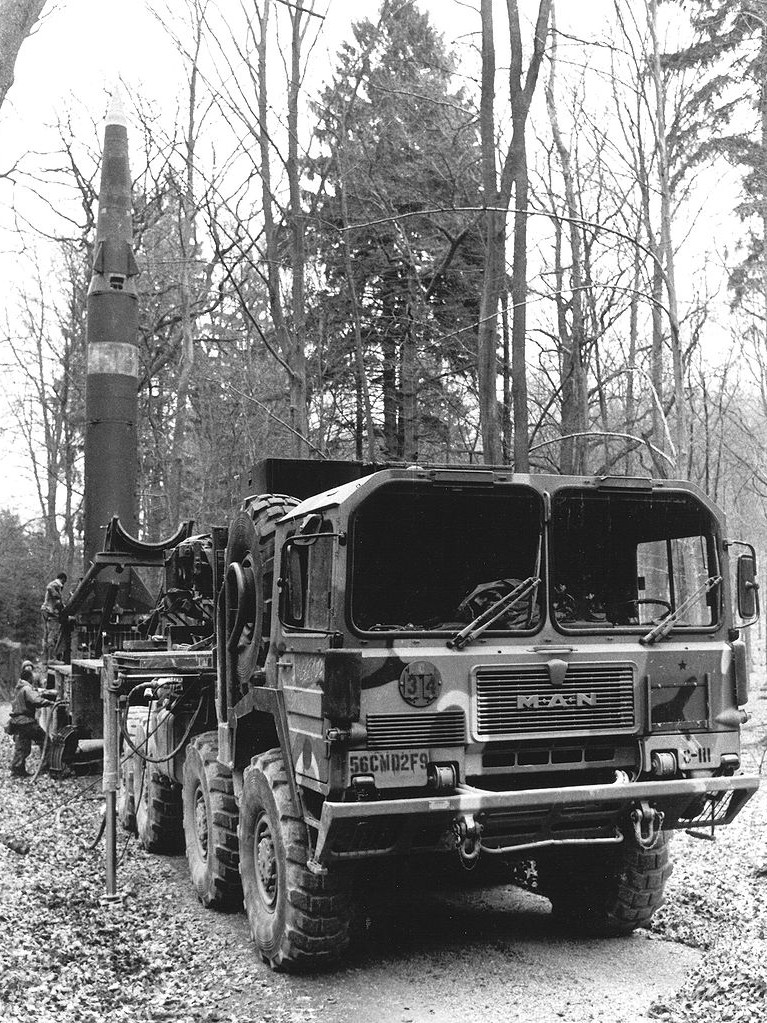
\includegraphics[width=2cm]{localimages/cc/weapons/797px-Pershing2MAN_ratio3-4.jpg}};

  \node<3-> [inner sep=0pt, font=\clf\vvtiny, anchor=south west, rotate=90] at (-0.8, -4) {Images: Nike Hercules - CC-BY August Freimuth, others - Public Domain, U.S. Federal Government works, downloaded from Wikimedia Commons};

%  \helpgridcornerdense[gray]
%  \helpgridcorner[black]
  
\end{tikzpicture}
\end{frame}
}

\note{Notes
NU - analytic tool, simplified map of nuclear weapon system

Missing things like Nike, ADM, artillery}

{
\usebackgroundtemplate{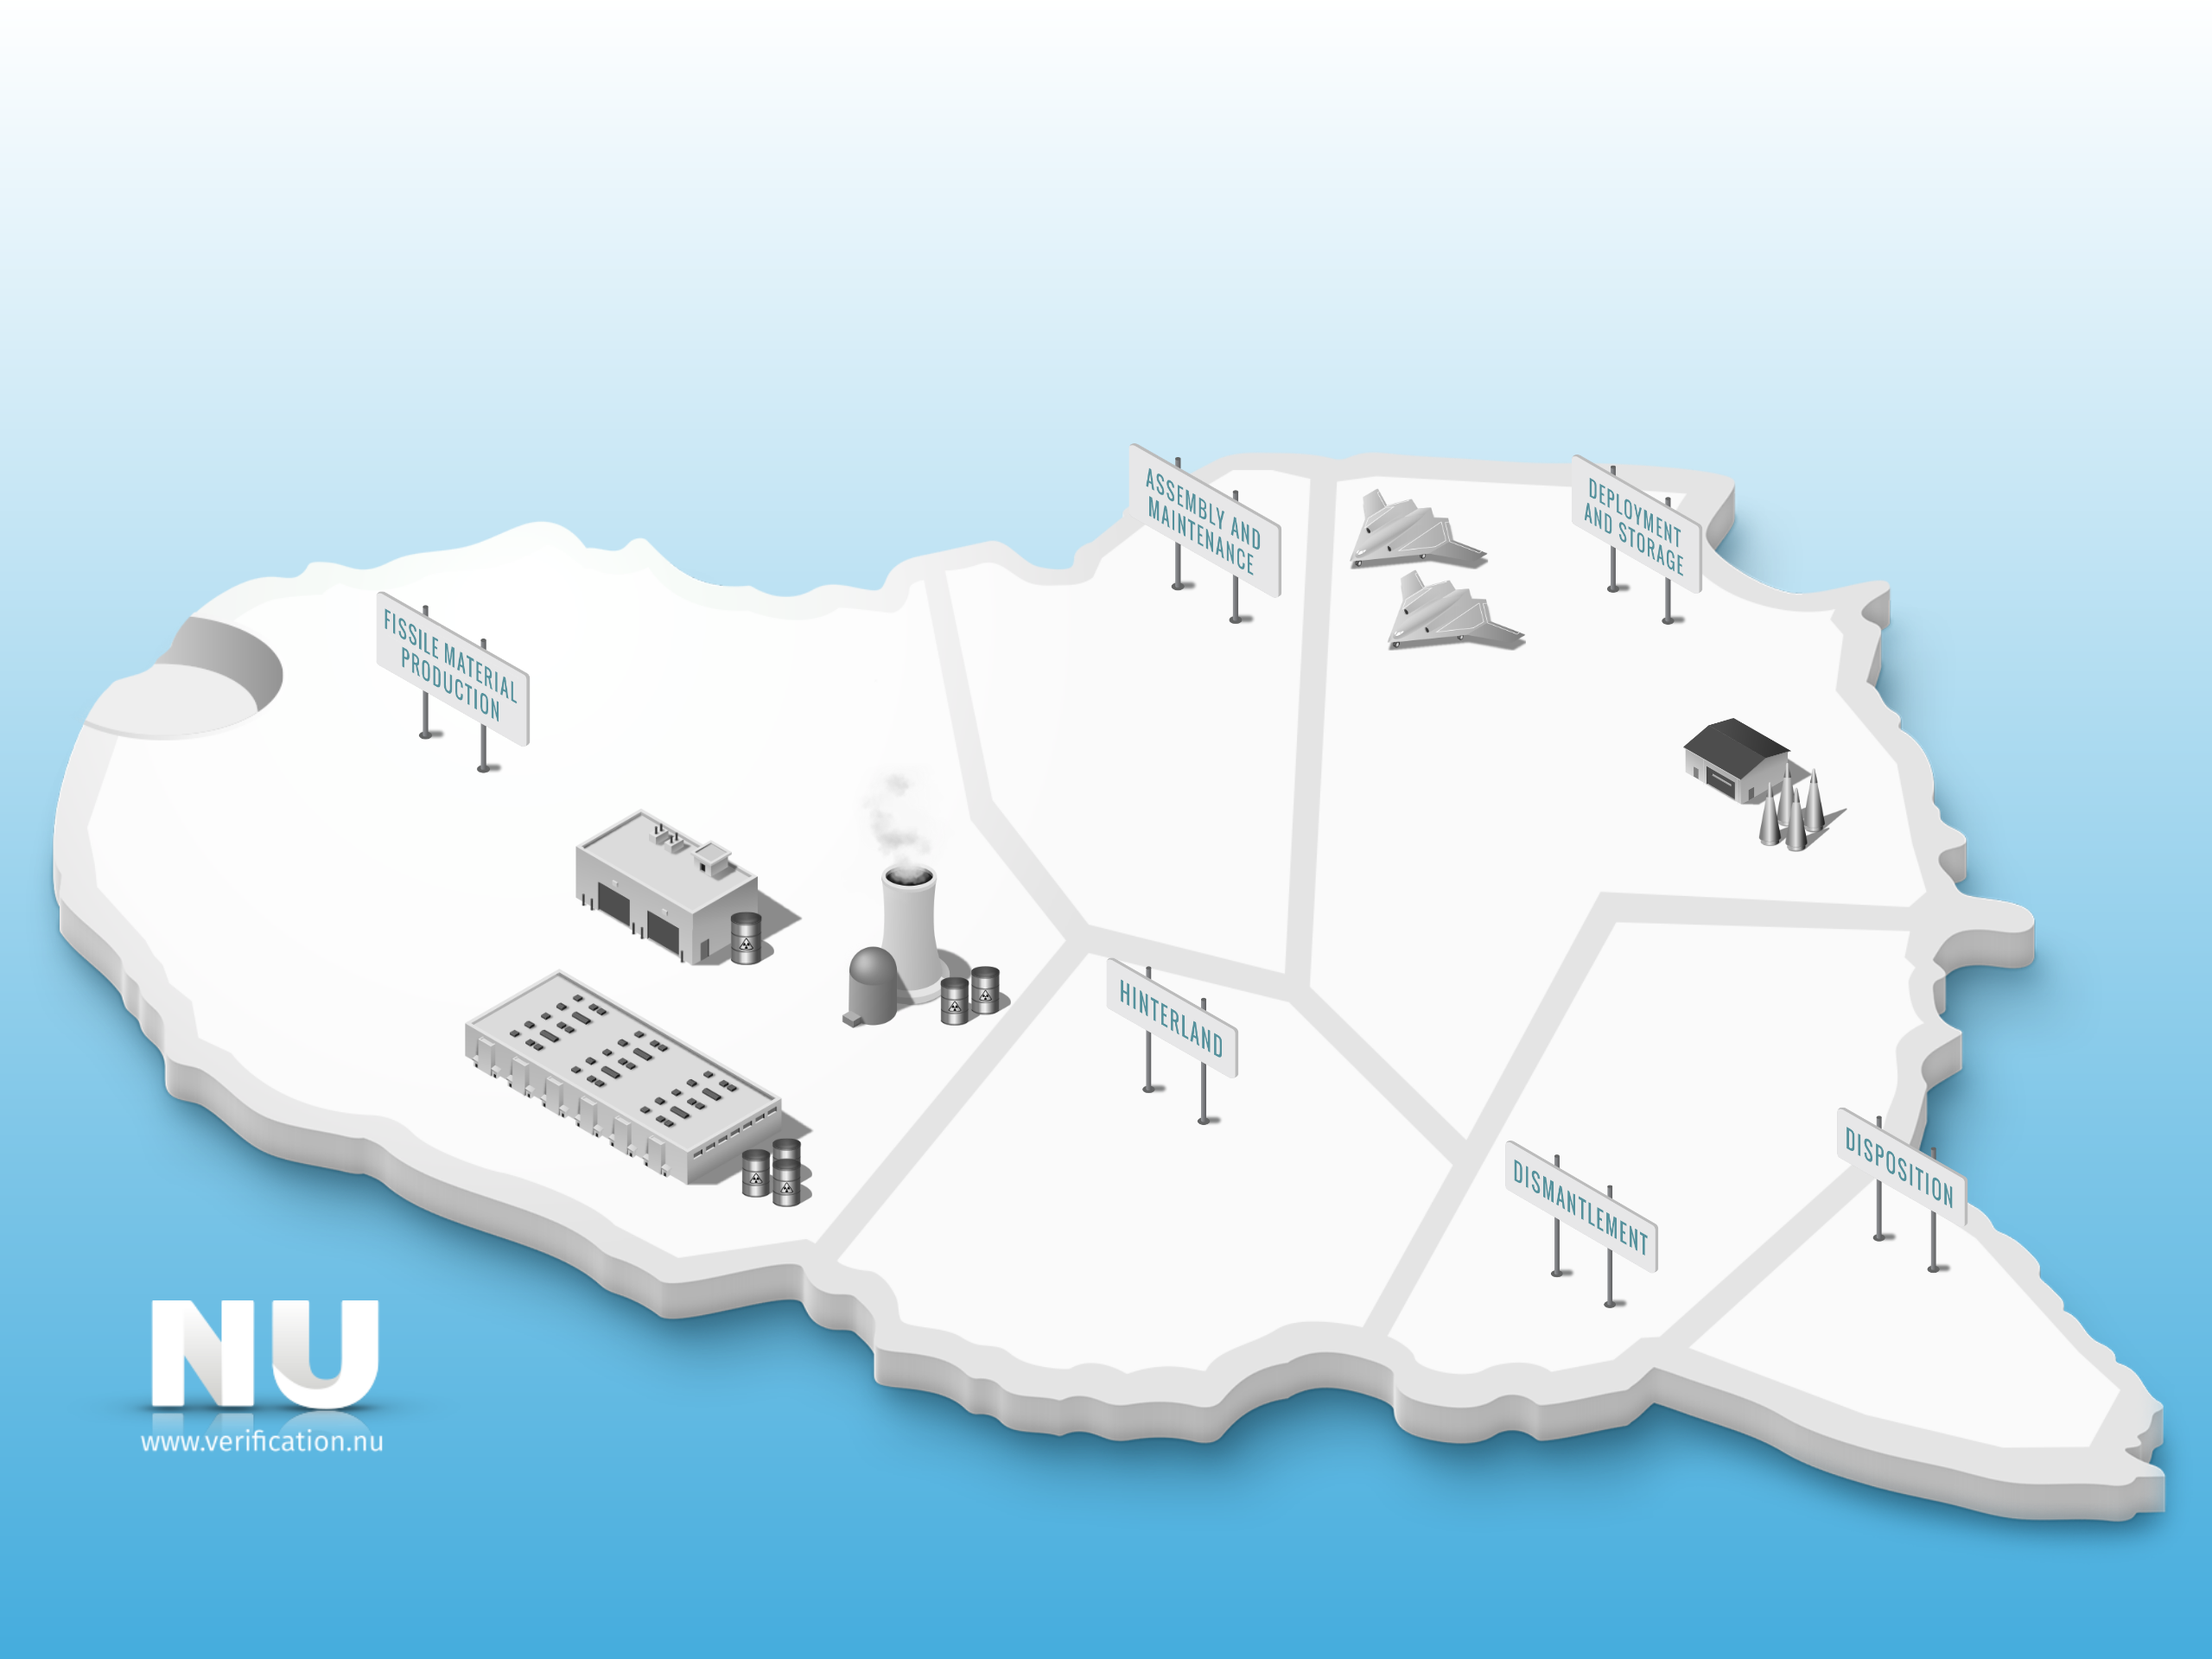
\includegraphics[width=\paperwidth]{localimages/cc/nu/germany/germany-2018.png}}
\begin{frame}{Germany Today}
  \begin{tikzpicture}[remember picture,overlay]
    \tikzset{cout/.style={
        rounded corners = 0.04cm,
        draw,
        text width=2.5cm,
        align=flush left,
        rectangle callout,
        fill=nuco,
        font=\scriptsize}};

  \node [cout, callout absolute pointer={(2.4,0.4)}, anchor=north] at (0.6,3.8) {
  \alert{Fuel Fabrication} \\ \usebeamercolor[fg]{normal text}
  \tiny
  Framatome operates a plant in Lingen with a capacity of 650tHM/y\\
  };
  \node [cout, callout absolute pointer={(2.2,-1.6)},anchor=north] at (0.6,-2.3) {\alert{Uranium Enrichment} \\ \usebeamercolor[fg]{normal text}
  \tiny
  URENCO operates a plant in Gronau with a capacity of 4,000 tSWU/a\\
};
  \node [cout, callout absolute pointer={(4.4,-1)}, anchor=north] at (3.7,-2.3) {
  \alert{Reactors} \\ \usebeamercolor[fg]{normal text}
  \tiny
  7 power reactors remain in operation, phase out planned\\
  8 research reactors};

  \node [cout, text width=5.5cm, callout absolute pointer={(8.5, 0.2)}, anchor=north] at (8.3,-2.3) {
  \alert{Tactical Nuclear Weapons} \\ \usebeamercolor[fg]{normal text}
  \tiny
  20 B61 gravity bombs in one location (Büchel air base)\\ 
};

\end{tikzpicture}
\end{frame}
}

{
\usebackgroundtemplate{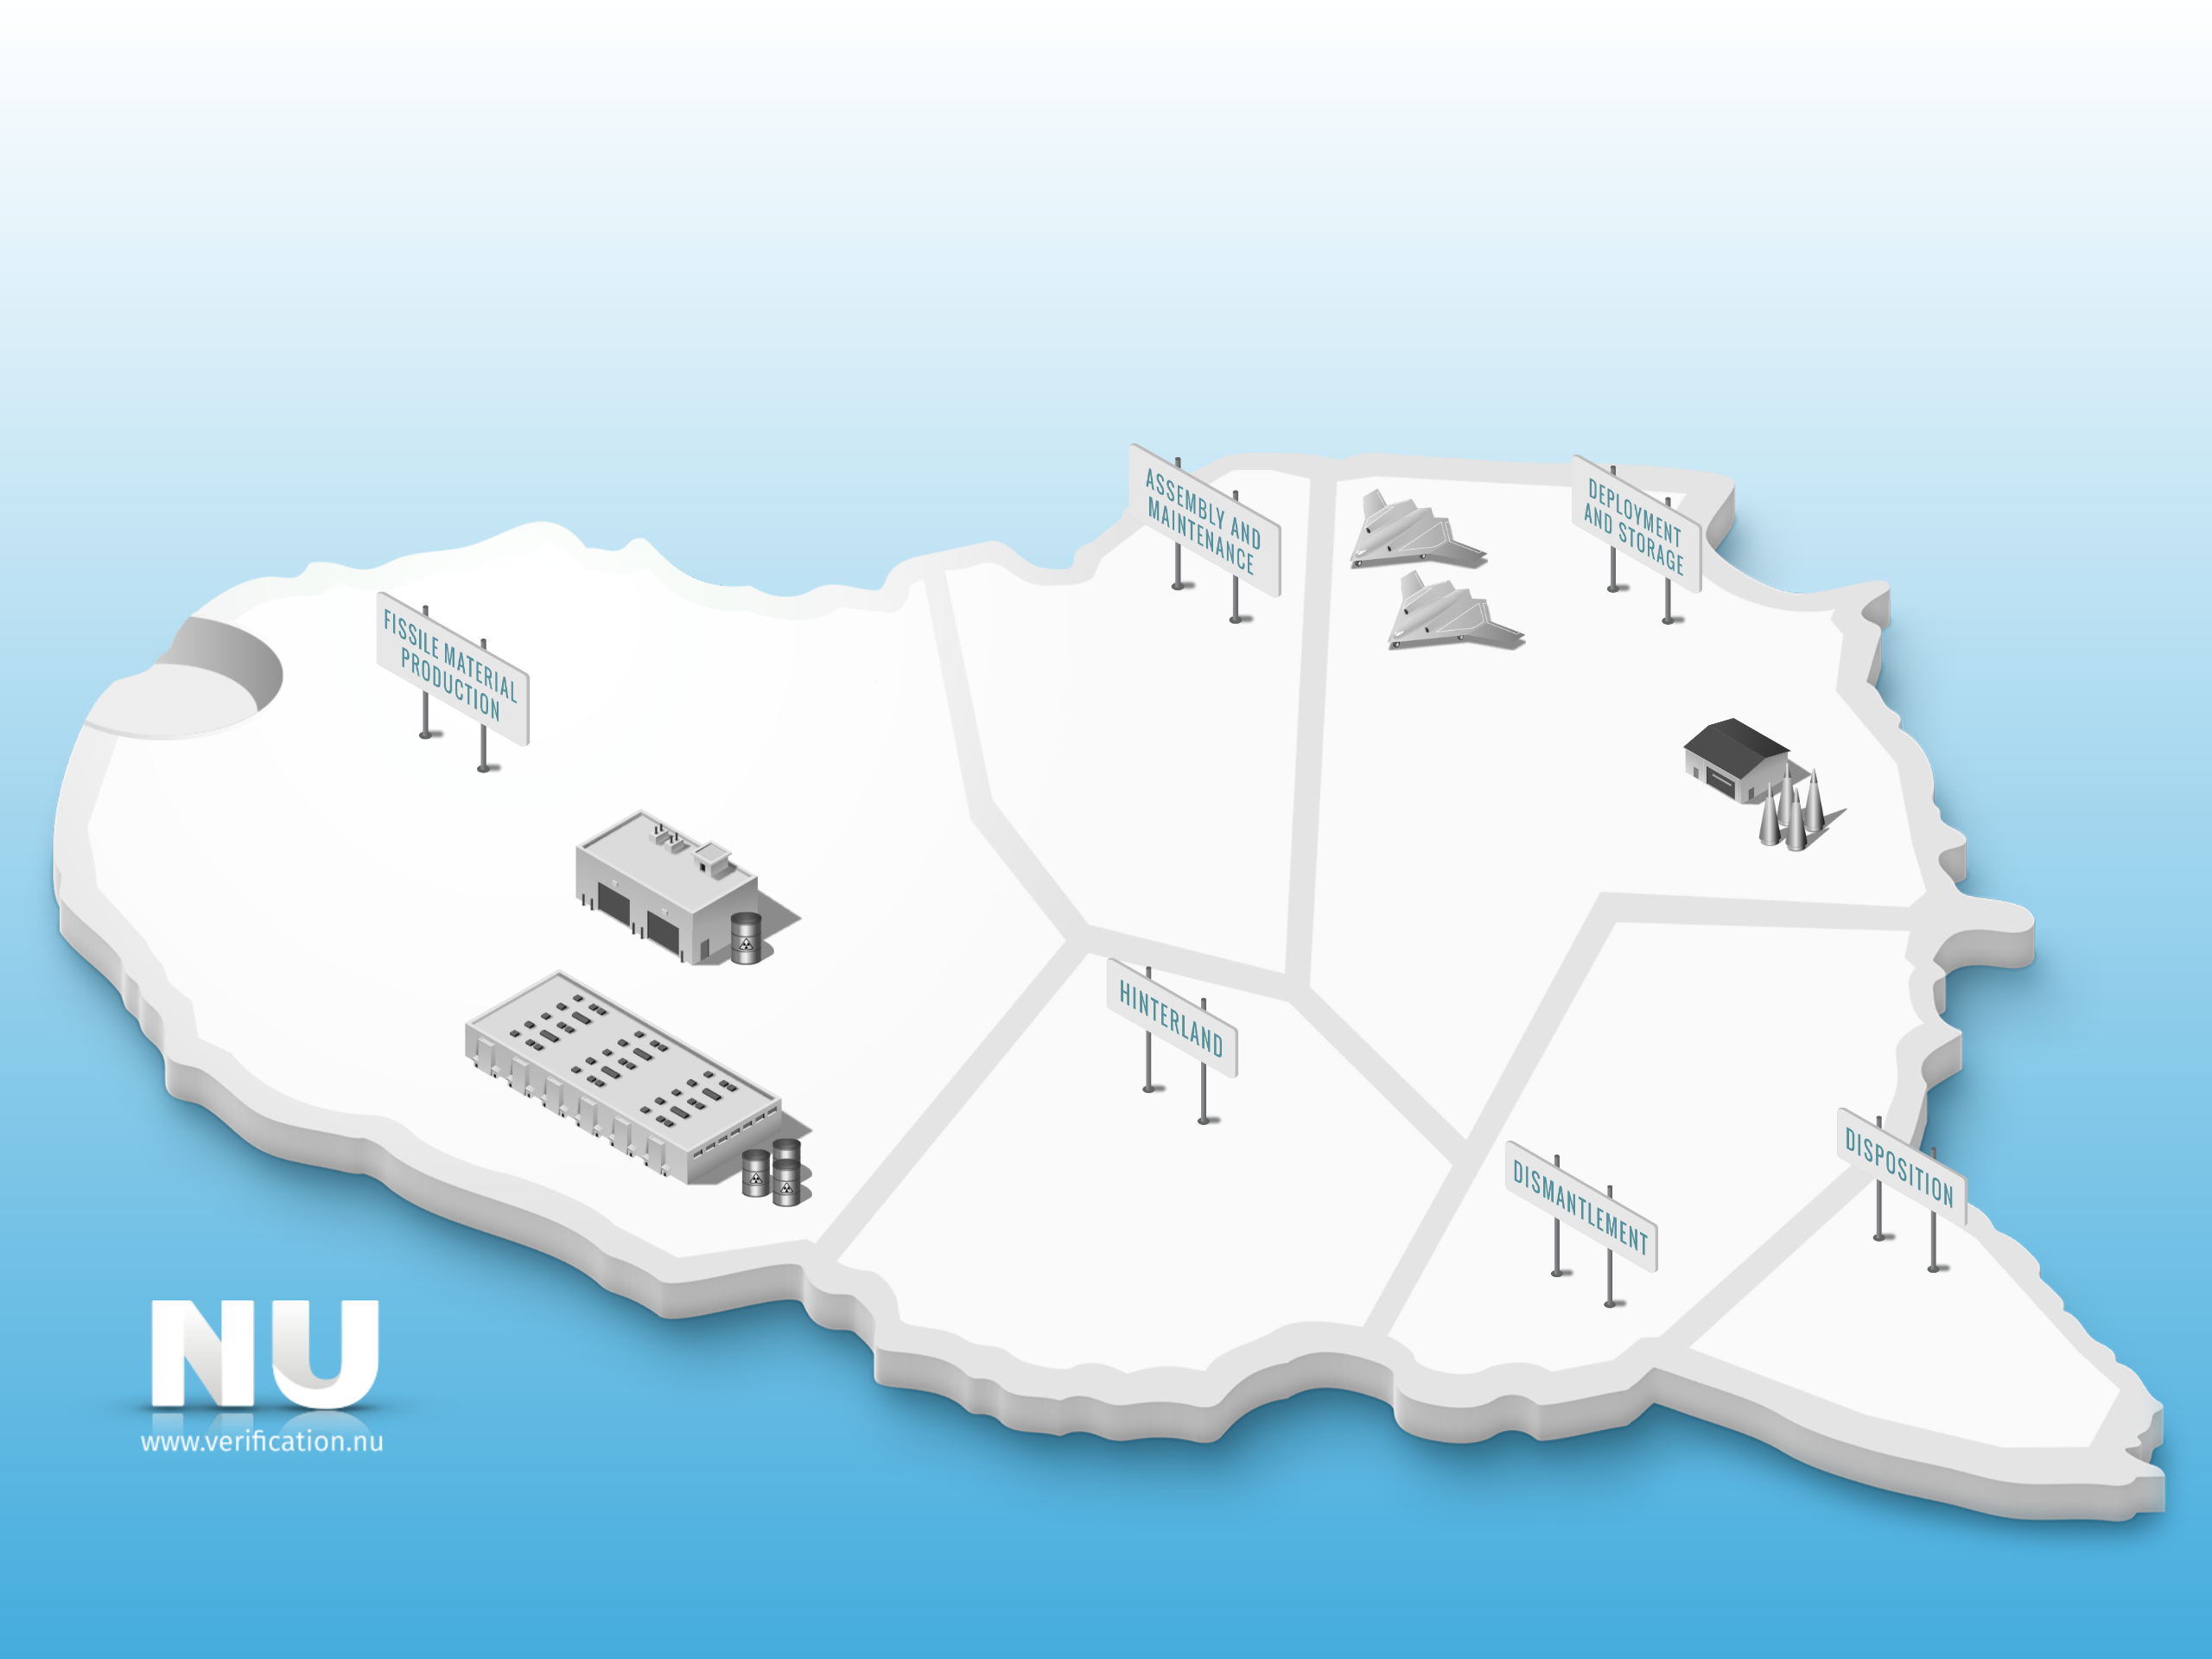
\includegraphics[width=\paperwidth]{localimages/cc/nu/germany/germany-2023.png}}
\begin{frame}{Nuclear Power Phase Out: 2023}
  \begin{tikzpicture}[remember picture,overlay]
    \tikzset{cout/.style={
        rounded corners = 0.04cm,
        draw,
        text width=2.5cm,
        align=flush left,
        rectangle callout,
        fill=nuco,
        font=\scriptsize}};

  \node [cout, callout absolute pointer={(2.4,0.4)}, anchor=north] at (0.6,3.8) {
  \alert{Fuel Fabrication} \\ \usebeamercolor[fg]{normal text}
  \tiny
  Framatome operates a plant in Lingen with a capacity of 650tHM/y\\
  };
  \node [cout, callout absolute pointer={(2.2,-1.6)},anchor=north] at (0.6,-2.3) {\alert{Uranium Enrichment} \\ \usebeamercolor[fg]{normal text}
  \tiny
  URENCO operates a plant in Gronau with a capacity of 4,000 tSWU/a\\
};
  \node [cout, callout absolute pointer={(4.4,-1)}, anchor=north] at (3.7,-2.3) {
  \alert{Reactors} \\ \usebeamercolor[fg]{normal text}
  \tiny
  Power reactors are shut down\\ Only research reactors remain\\};

  \node [cout, text width=5.5cm, callout absolute pointer={(8.5, 0.2)}, anchor=north] at (8.3,-2.3) {
  \alert{Tactical Nuclear Weapons} \\ \usebeamercolor[fg]{normal text}
  \tiny
  20 B61 gravity bombs in one location (Büchel air base)\\ 
};

\end{tikzpicture}
\end{frame}
}

{
\usebackgroundtemplate{
\includegraphics[width=\paperwidth]{localimages/cc/nu/germany/germany-goal.png}}
\begin{frame}[t]{A Future Goal?}
\small 
With a shrinking world nuclear energy market (and no domestic requirements), uranium enrichment and fuel fabrication facilities could be closed.

\begin{tikzpicture}[remember picture, overlay]
  \tikzset{shift={($(current page.center) - (5.4, 0.3)$ )}};
  \tikzset{cout/.style={
        rounded corners = 0.04cm,
        draw,
        text width=2.5cm,
        align=flush left,
        rectangle callout,
        fill=nuco,
        font=\scriptsize}};
  \node [cout, callout absolute pointer={(4.4,-1)}, anchor=north] at (3.7,-2.3) {
  \alert{Research Reactors} \\ \usebeamercolor[fg]{normal text}
  \tiny
  (No HEU fuel)\\};

\end{tikzpicture}

\end{frame}
}

\note {
Fuel Fabrication / Enrichment closure discussed by outgoing minister for environment barbara hendricks

Legal Study undertaken, published in November 2017

Problem: Treaty of Almelo. Apparently Germany could leave the treaty within a years time.
}


\section{More on Tactical Nuclear Weapons}
\label{sec:orgf17d8b2}

\begin{frame}[label={sec:org0e4bf18}]{Origins of NATO Nuclear Sharing}
\begin{block}{North Atlantic Treaty (1949)}
No statements with regard to nuclear weapons
\end{block}
\begin{block}{First Strategic Concept (1949)}
\emph{Insure the ability to carry out strategic bombing including the prompt delivery of the atomic bomb. This is primarily a U.S. responsibility assisted as practicable by other nations.} \\[0.1em]

\raggedleft \vtiny M.C. 3/2, Note by the Secretary to the North Atlantic Military Commitee on the Strategic Concept for the Defense of the North Atlantic Area, 1949, p. 23

\pause
\end{block}
\begin{block}{North Atlantic Council Meeting (1957)}
\emph{To this end, NATO has decided to establish stocks of nuclear warheads, which will be readily available for the defence of the Alliance in case of need.} \\[0.1em]

\hfill \vtiny Final Communiqué, Chairman: Mr. P.H. Spaak, Secretary General of NATO, December 16 1957
\end{block}
\begin{block}{Defense and Deterrence Posture Review (2012)}
\emph{As long as nuclear weapons exist, NATO will remain a nuclear alliance.}

\emph{[\ldots{}] seeking to create the conditions and considering options for further reductions of non-strategic nuclear weapons [\ldots{}]}

\hfill \vtiny NATO, 'Deterrence and Defence Posture Review', 2012
\end{block}
\end{frame}


\begin{frame}[label={sec:orge7e1105}]{Today: Only one site}
\vspace{-0.8cm}
\begin{center}
\LARGE 
20 B61 gravity bombs, Fliegerhorst Büchel
\end{center}

\begin{columns}[T]
\begin{column}{0.5\columnwidth}
\begin{imageboxplain}
  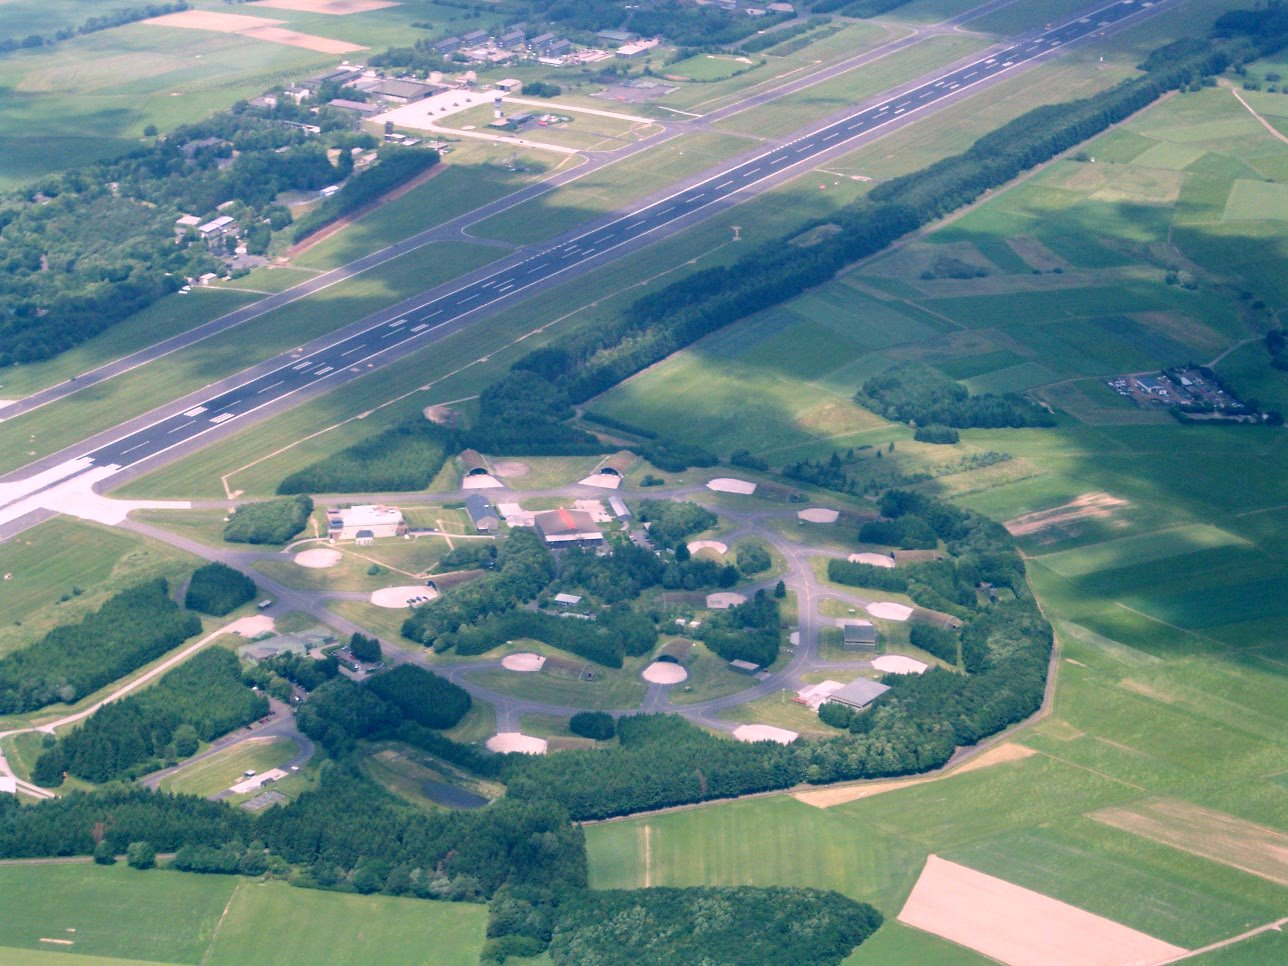
\includegraphics[width=\textwidth]{localimages/cc/places/Buechel_Fliegerhorst.jpg}
\end{imageboxplain}
\end{column}
\begin{column}{0.5\columnwidth}
\small

Büchel is a German Airbase in Rheinland Pfalz since 1958, hosts the \\"Taktische Luftwaffengeschwader 33"\\[0.4em]

B61 gravity bombs are to be delivered with German Tornado aircraft \\[0.4em]

Weapons are stored in vaults in hangars "Weapon Storage and Security System" (WS3)
\end{column}
\end{columns}



\begin{tikzpicture}[remember picture, overlay]
  \tikzset{shift={($(current page.center) - (5.4, 0.3)$ )}};

  \node [anchor=south west, rotate=90, font=\vvtiny] at (-0.3, -2) {Image Source: CC-BY-SA 3.0, Stahlkocher, Wikimedia Commons};
  
  % \helpgridcornerdense[gray]
  % \helpgridcorner[black]
\end{tikzpicture}
\end{frame}

\begin{frame}[standout,label={sec:orgb862e8a}]{}
What would be a credible scenario of use?

\note{
Tact nukes Useless (especially after 2020/25)
}
\end{frame}


{
\usebackgroundtemplate{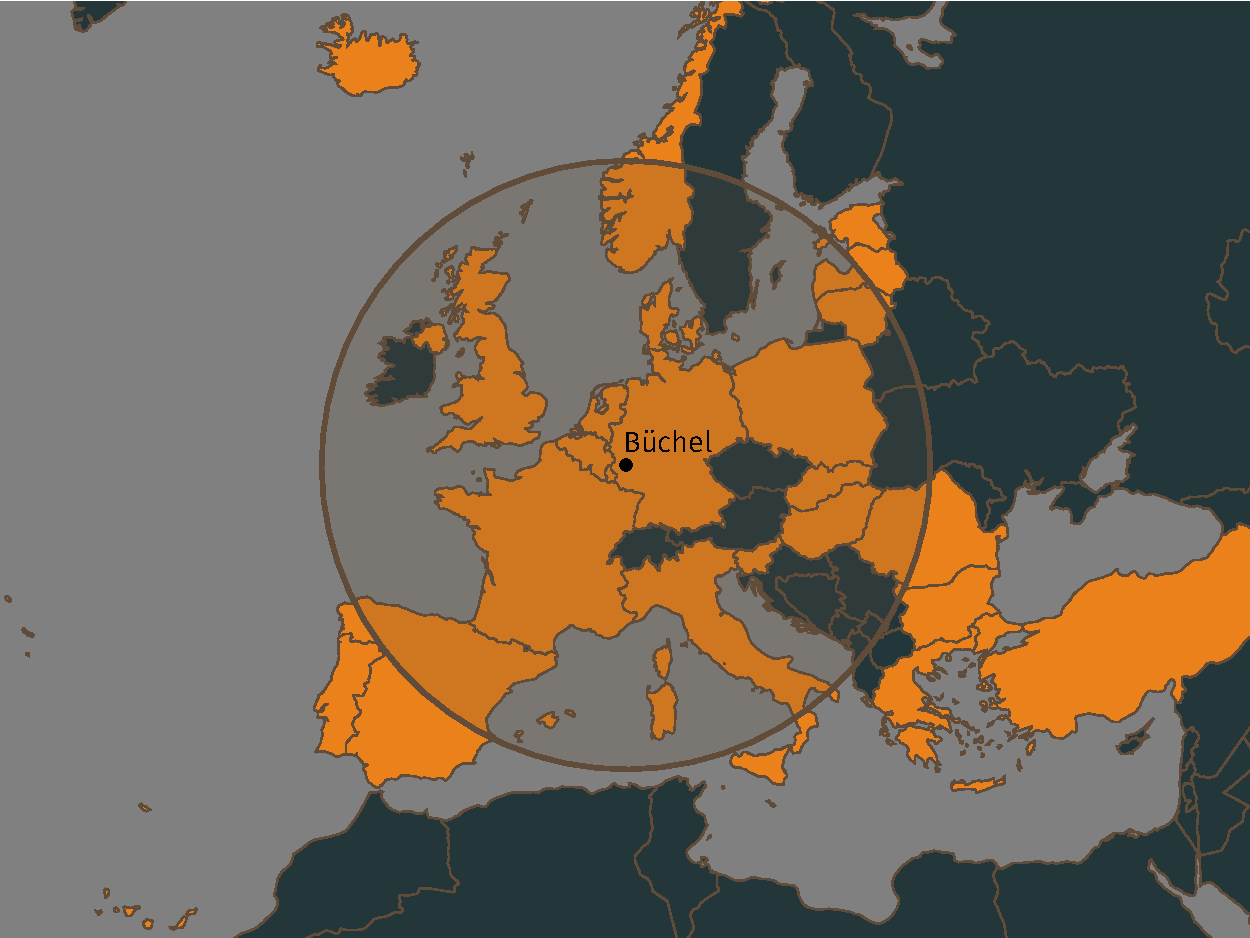
\includegraphics[width=\paperwidth]{localimages/own/maps/tornado.pdf}}
\begin{frame}[t,label={sec:org3c8dc83}]{}
\vspace{0.7cm}
   \textbf{Tornado has an operating\\
   radius of 1390 km}
\end{frame}

}


{
\usebackgroundtemplate{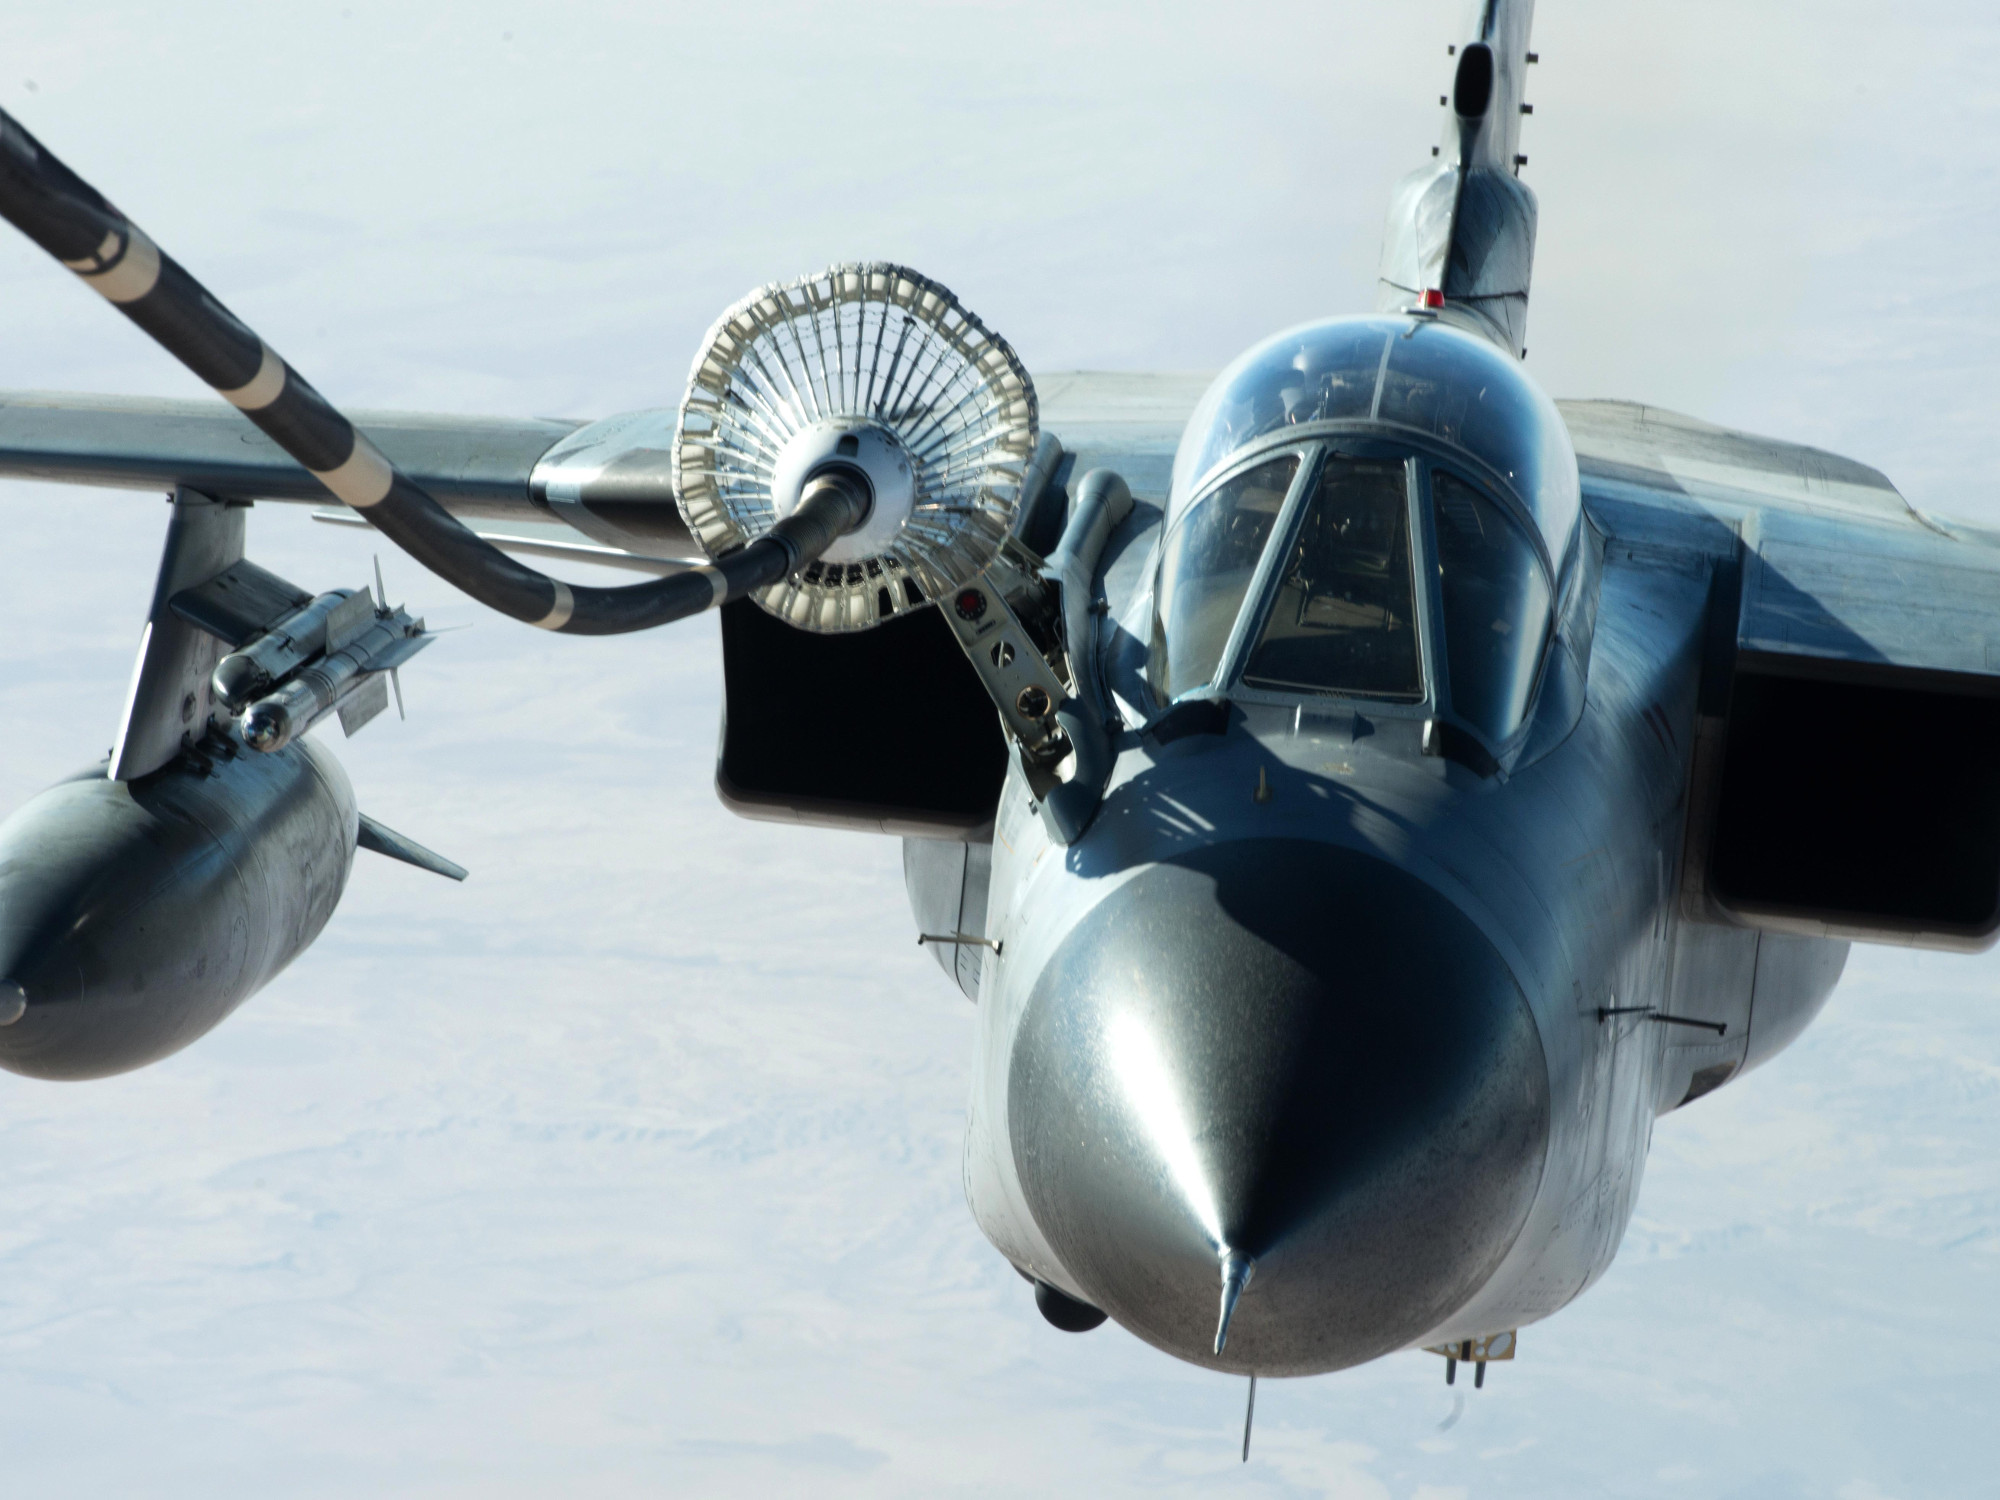
\includegraphics[width=\paperwidth]{localimages/cc/deliverysystems/German_Tornado_refuelled_by_KC-10_ratio4-3.jpg}}
\begin{frame}[label={sec:org6a49855}]{}
\begin{tikzpicture}[remember picture, overlay]
  \tikzset{shift={($(current page.center) - (5.4, 0.3)$ )}};
  
  \node[anchor=north west, text width=6cm, align=flush left] at (-0.6, -1.8) {
  Longer missions require refueling, which can only be done by aircrafts of other countries.
  };
  \node [anchor = south west, font=\clf\vtiny] at (-0.6, -4.4) {Image: Public Domain, U.S. Air Force photo/Staff Sgt. R. Alex Durbin};
  
  % \helpgridcornerdense[gray]
  % \helpgridcorner[black]
\end{tikzpicture}

\note{
Refueling of Tornados is technically possible.
Germany does not have large tankers.
Tornado to Tornado refueling is possibility, but limited in range.
Apparently, refueling from other aircraft was only part of a 1995 training in preparation for NATO missions, Germany paid for it (Tornado book)
}
\end{frame}

}


\begin{frame}[label={sec:orge9be90d}]{Outdated and Error Prone}
\begin{center}

End-of-life for Tornado aircraft soon, probably 2025.

Last year, only 26 of 93 Tornado aircraft were combat-ready.\\[1em]

\begin{tornpagetb}[fill=white]{top=0pt,bottom=0pt,width=0.9\textwidth}
  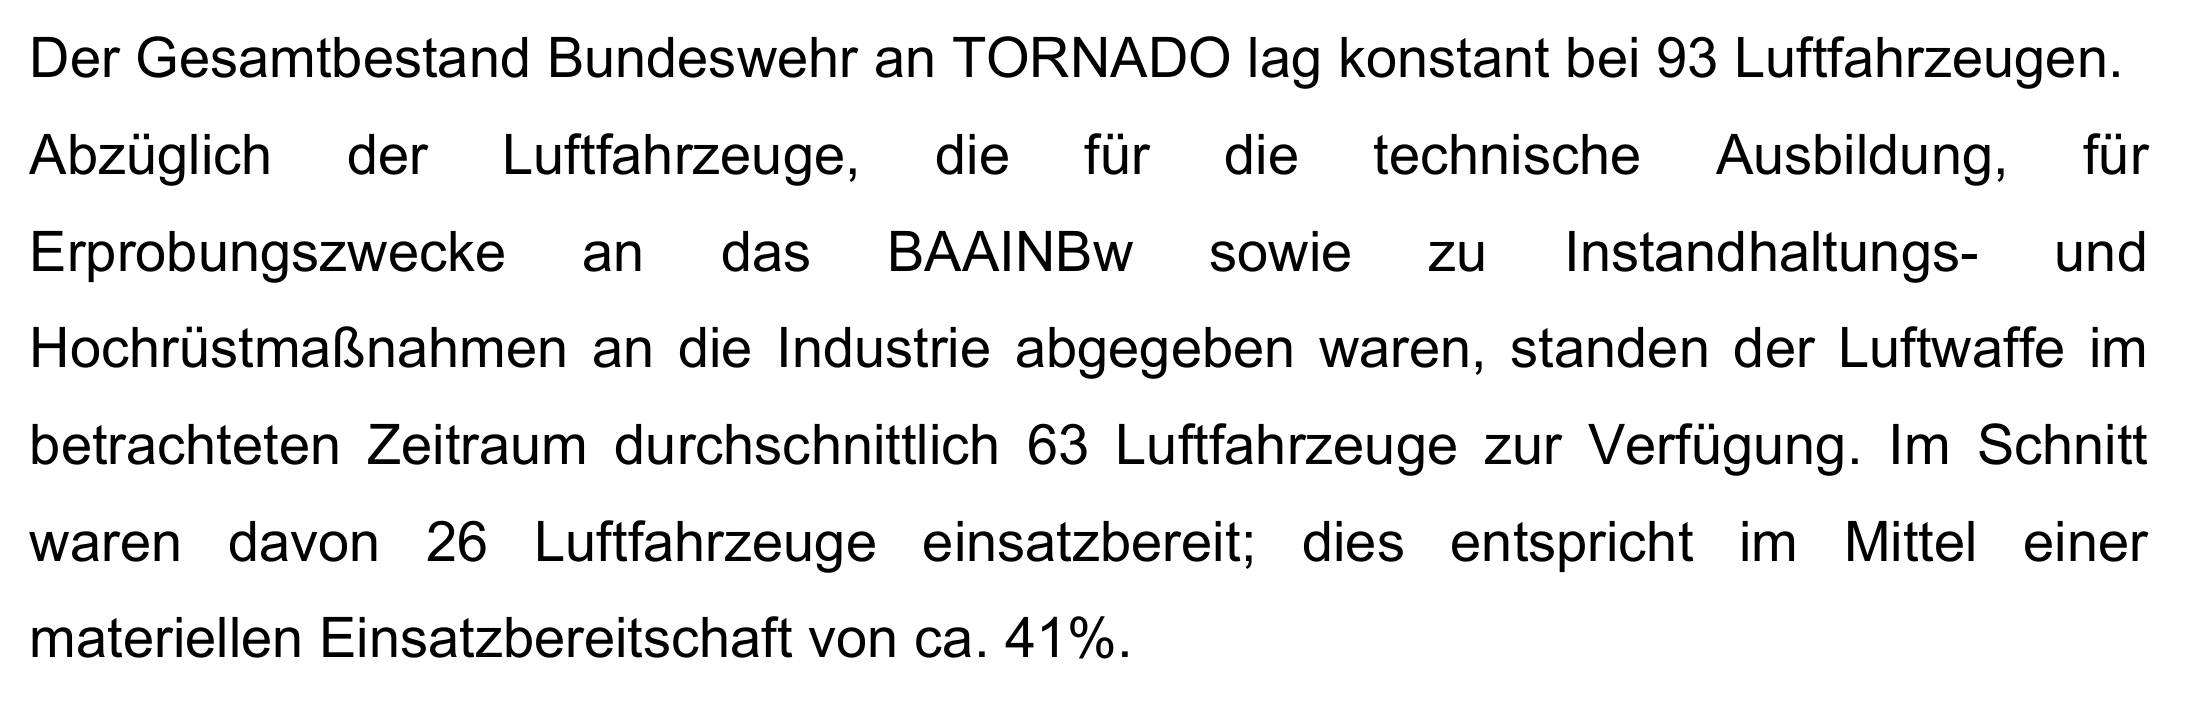
\includegraphics[width=\textwidth]{localimages/quotes/BMV-2018-tornado.png}
\end{tornpagetb}
\scriptsize "Bericht zur materiellen Einsatzbereitschaft der Hauptwaffensysteme der Bundeswehr 2017", German Ministry of Defense, February 2018.


\end{center}
\end{frame}

\begin{frame}[label={sec:org387a213}]{Replacement Options}
\begin{imagebox2rows}[lefthand width=3.75cm]{images/cc/deliverysystems/1600px-German_eurofighter_ratio5-4.jpg}
\alert{Eurofighter} \\
\scriptsize
European cooperative project by multinational Eurofighter Jagdflugzeug GmbH, Germany currently owns 128 planes\\[0.1em]
None is capable to carry the B61(-12), and adjustments are unlikely
\end{imagebox2rows}

\begin{imagebox2rows}[lefthand width=3.75cm]{images/cc/deliverysystems/1600px-F-35A_flight_(cropped)_ratio5-4.jpg}
\alert{F35} \\
\scriptsize
US fighter jet by Lockheed Martin \\[0.1em]
Produced in the US, and in Italy \\[0.1em]
Capability to deliver B61-12 (planned)
\end{imagebox2rows}

\vvtiny Image Sources (top to bottom): \\CC-BY-SA 3.0, Krasimir Grozev / Wikimedia Commons; \\Public Domain, U.S. Air Force photo by Master Sgt. Donald R. Allen / Wikimedia Commons

\note{
after italian elections: 5 start movement wants to get rid of italian f35 production (and use
}
\end{frame}





\section{Political Situation in Germany}
\label{sec:orgde7a51b}
\begin{frame}[label={sec:org79cf193}]{Government Position (on Tactical Nuclear Weapons)}
\small

Deterrence is necessary as long as nuclear weapons \\ can be means of military conflicts

NATO is a nuclear alliance

Through nuclear sharing, Germany can remain part of NATO's nuclear planning

\onslide<2->{
\alert{Commited to establish conditions for a world free of nuclear weapons}
}

\vspace{0.6cm}
\vfill

\begin{tornpagetb}[fill=white]{top=0pt,bottom=0pt,halign=flush left,fontupper=\tiny}
Solange nukleare Waffen ein Mittel militärischer Auseinandersetzungen sein können, besteht die Notwendigkeit zu nuklearer Abschreckung fort. Die strategischen Nuklearfähigkeiten der Allianz, insbesondere die
der USA, sind der ultimative Garant der Sicherheit ihrer Mitglieder. Die NATO ist weiterhin ein nukleares Bündnis. Deutschland bleibt über die nukleare Teilhabe in die Nuklearpolitik und die diesbezüglichen
Planungen der Allianz eingebunden. Dies geht einher mit dem Bekenntnis Deutschlands zu dem Ziel, die
Bedingungen für eine nuklearwaffenfreie Welt zu schaffen.
\end{tornpagetb}
\scriptsize 
\hfill Weißbuch 2016 zur Sicherheitspolitik und zur Zukunft der Bundeswehr, p. 65

\note{
As long as nuclear weapons can be means of military conflicts, nuclear deterrence remains necessary.
[\ldots{}]
This goes along with Germany's commitment to the goal of achieving the conditions for a nuclear weapon free world.
(own translation, Weißbuch 2016 zur Sicherheitspolitik und zur Zukunft der Bundeswehr, p. 65)


JANUS HEAD needed!
}
\end{frame}

\begin{frame}[label={sec:org564b299}]{Government Position (on Ban Treaty)}
\begin{exampleblock}{Again}
Support for the goal of a world without nuclear weapons and concrete nuclear disarmament steps
\end{exampleblock}

\begin{alertblock}{But There are Concerns}
Ban Treaty is a danger for NPT and related non-proliferation and disarmament regime

States could see Ban Treaty as an alternative, therefore leave the NPT

Special concern: Verification (Lower verification standards as compared to NPT)
\end{alertblock}

\vspace{0.7cm}

\begin{tornpagetb}[fill=white]{top=0pt,bottom=0pt,halign=flush left,fontupper=\tiny}
Die Bundesregierung teilt und unterstützt das Ziel einer Welt ohne Nuklearwaffen.  Wir stehen aktiv für dieses Ziel ein, indem wir uns entschieden für konkrete nukleare Abrüstungsschritte einsetzen. 
[\ldots{}]
Der  aktuell  verhandelte  Verbotsvertrag  ist  nach  Ansicht  der  Bundesregierung  nicht  förderlich,  um  dem  Ziel  einer  nuklearwaffenfreien  Welt  näher  zu  kommen. Im  Gegenteil,  ein  solcher  Ansatz  droht  dem  bestehenden, von 191 Staaten Ratifizierten Nuklearen Nichtverbreitungsvertrag  (NVV)  und  dem  mit  ihm  verbundenen Kontrollregime  zur  Verhinderung  nuklearer  Proliferation  nachhaltigen  Schaden  zuzufügen  sowie  das  globale Nonproliferations- und Abrüstungsregime zu gefährden. Denn es kann nicht ausgeschlossen werden, dass Staaten einen Verbotsvertrag als Alternative zum NVV ansehen, im schlimmsten Fall letzteren verlassen könnten. Unsere  Besorgnis  gilt  insbesondere  der  wichtigen Frage  der  Verifikation:  Nach  derzeitigem  Stand  droht das  geplante  Atomwaffenverbot  hinter  die  heute  vorherrschenden Verifikationsstandards der Internationalen Atomenergie-Organisation  (IAEO)  und  der  NVV-Vertragsstaaten  zurückzufallen  und  dadurch  den  NVV  zu schwächen.
\end{tornpagetb}
\scriptsize 
\hfill Dr. Maria Böhmer (Staatsministerin), Bundestagsprotokoll 18/239, Plenary Meeting, June 21, 2017.
\end{frame}


\begin{frame}[label={sec:org73db639}]{(Selected) Foreign Ministers}
\begin{imagebox3rows}[fontlower=\scriptsize,lefthand width=2.1cm]{images/cc/people/1024px-Westerwelle_hamm_2009_square.jpg}
\alert{Guido Westerwelle, FDP †} \\
\tinyscriptsize
Removal of tactical nuclear weapons was one of his key policy initiatives \\[0.2em]
Initiated (with colleagues) NATO discussion that lead to Chicago Summit 2012 declaration
\end{imagebox3rows}

\begin{imagebox3rows}[fontlower=\scriptsize,lefthand width=2.1cm]{images/cc/people/2017-03-19_Sigmar_Gabriel_SPD_Parteitag_by_Olaf_Kosinsky-3_square.jpg}
\alert{Sigmar Gabriel} \\
\tinyscriptsize
While still being foreign minister, he supported SPD's chancellor candidate Martin Schulz, who anounced removal of tactical nuclear weapons as part of his campaign  \\[0.2em]
\end{imagebox3rows}

\begin{imagebox3rows}[fontlower=\scriptsize,lefthand width=2.1cm]{images/cc/people/2017-03-26_Heiko_Maas_by_Sandro_Halank–1_square.jpg}
\alert{Heiko Maas} \\
\tinyscriptsize
Designated new foreign minister, previously head of ministry of justice \\[0.2em]
No public position on tactical nuclear weapons (yet)
\end{imagebox3rows}

\vvtiny Image Sources (top to bottom): \\
 CC-BY 3.0, Dirk Vorderstraße/Wikimedia Commons; \\
CC-BY-SA 3.0, Olaf Kosinsky / kosinsky.eu; \\
CC-BY-SA 3.0, Sandro Halank, Wikimedia Commons.
\end{frame}

\begin{frame}[label={sec:org1db9d29}]{Political Parties (2017 Federal Elections)}
\begin{tikzpicture}[remember picture, overlay]
  \tikzset{shift={($(current page.center) - (5.4, 0.3)$ )}};
  \tikzset{cparty/.style={
  font=\tinyscriptsize\slshape,
  fill=white,
  text width=4cm, 
  align=flush left,
  fill opacity=0.9,
  rounded corners,
  text opacity=1,
  }};
  \tikzset{oparty/.style={
  cparty,
  text width=6cm
  }};
  \tikzset{orparty/.style={
  cparty,
  text width=5cm
  }};
  \tikzset{titlep/.style={draw, drop shadow, fill=white,inner sep=0pt}}

  \node (ctreaty) [at=(current page.center), shift={(0, 2cm)}, minimum width=2cm, minimum height=3.1cm] {};

  \node (spd) [titlep, rotate=10, left = 1cm of ctreaty] {
\includegraphics[page=1, width=2cm]{localimages/quotes/wp2017-spd-cover.pdf}};

  \node (spd text) [at = (spd),cparty] {SPD: "A world without Nuclear Weapons and other WMDs remains our goal. [...] We stand for the withdrawal of tactical nuclear weapons from Germany and Europe as part of a European disarmament treaty."};

  \node (cdu) [titlep, right = 1cm of ctreaty, rotate=-10] {
\includegraphics[page=1, width=2cm]{localimages/quotes/wp2017-cducsu-cover.pdf}};
  
  \node<1>  (cdu text) [at=(cdu),cparty] {CDU: Nothing for 2017 };
  \node<2-> (cdu text 2) [at=(cdu),orparty] {CDU: Nothing for 2017. \\ 2013: "We will support every initiative to reduce nuclear weapons and limit conventional forces that is fair and serves international security. An agreement on drastic reductions of nuclear weapons creates the prospect to strengthen the regime for non-proliferation of WMD [...]" };


  \node (linke) [titlep, below left = 0.2cm and 3.5cm of ctreaty, rotate=10] {
\includegraphics[page=1, width=1.5cm]{localimages/quotes/wp2017-linke-cover.pdf}};
  \node (gruene) [titlep, below left = 2.2cm and -1.8cm of ctreaty,rotate=-10] {
\includegraphics[page=1, width=1.5cm]{localimages/quotes/wp2017-gruene-cover.pdf}};

  \node (linke text) [at=(linke.east),shift={(1.5cm,-0.2cm)},cparty] {Linke: The last US nuclear weapons stationed in germany must be removed and destroyed immediately. [...] DIE LINKE stands for a the abolition of nuclear weapons under international treaties.};
  \node (gruene text) [at=(gruene.west),shift={(-1.9cm,-0.8cm)},oparty] {Grüne: "Worldwide disarmament must become a cornerstone of German and European foreign policy - especially in troubling times. We fight for a world without nuclear weapons and to outlaw them by an international convention. [...] We demand withdrawal of the nuclear weapons in Büchel and final abandoning of 'nuclear sharing'.};

  \node (fdp) [titlep, below right = 0.4cm and 0.1cm of ctreaty,rotate=10] {
\includegraphics[page=1, width=1.5cm]{localimages/quotes/wp2017-fdp-cover.pdf}};

  \node (afd) [titlep,below right = 2.6cm and 3.5cm of ctreaty, rotate=-20] {
\includegraphics[page=1, width=1.5cm]{localimages/quotes/wp2017-afd-cover.pdf}};

  \node (fdp text) [at=(fdp.east),shift={(1cm,-0.2cm)},cparty] {FDP: "We need [...] a new diplomatic approach for arms control and disarmament. Germany and its close partners should take a leading role in this." (p. 105)};
  \node (afd text) [at=(afd.west),shift={(-0.8cm,-0.8cm)},orparty] {AfD: "The AfD stands for the withdrawal of all allied troops stationed on German soil, and especially their nuclear weapons." (p. 31)};
  
  
  % \helpgridcornerdense[gray]
  % \helpgridcorner[black]
\end{tikzpicture}
\tinyscriptsize
\end{frame}

\begin{frame}[label={sec:orgef7bd94}]{(Some) Civil Society Actors}
\begin{block}{ICAN Germany}
Part of ICAN, formally organized since 2014, based mostly in Berlin.
\end{block}

\begin{block}{IPPNW Germany}
National branch of IPPNW, founded in 1982.
\end{block}

\begin{block}{Trägerkreis Atomwaffen abschaffen}
Longstanding collaboration between various local groups. Most prominent campaign in recent past was "atomwaffenfrei.jetzt!".
\end{block}

\begin{block}{Heinrich Böll Stiftung}
Political foundation, close to Bündnis 90/Grüne. Supports research work of ICAN Germany.
\end{block}
\end{frame}


\begin{frame}[label={sec:org10ca172}]{Public Opinion}
\begin{center}
\Large

\ldots{}depends on the question asked.\\[1.5em]

\small

Recent ICAN Germany survey:\\
71\% for ban, 14\% against, 15\% undecided

\end{center}

\hfill \tiny Source for Survey: icanw.de
\end{frame}

\section{Treaty on the Prohibition of Nuclear Weapons (Ban Treaty)}
\label{sec:org0af576b}

\begin{frame}[label={sec:org3f505f6}]{Relevant Articles}
%\tcbset{enhanced, fuzzy halo=fg, sharp corners, center}
\setbeamertemplate{enumerate subitem}{(\alph{enumii})}
\tcbset{enhanced, colback=white, sharpish corners, fuzzy halo=0.5mm with fg,boxrule=0pt}
\begin{tcolorbox}[center, width=0.8\textwidth]
\scriptsize
\centering
Article 1\\
Prohibitions
\tinyscriptsize
\begin{enumerate}
\item Each State Party undertakes never under any circumstances to:

\begin{enumerate}
\tinyscriptsize
%\setcounter{enumii}{1}\item \textcolor<1>{gray!20}{\color<2->{gray!20}Develop, test, produce, manufacture, otherwise acquire, possess or stockpile nuclear weapons or other nuclear explosive devices;}
\setcounter{enumii}{1}\item \textcolor<1-3>{gray!20}{\color<3->{fg}Transfer to any recipient whatsoever nuclear weapons or other nuclear explosive devices or control over such weapons or explosive devices directly or indirectly;}
\setcounter{enumii}{2}\item \textcolor<1-3>{gray!20}{\color<3->{fg}Receive the transfer of or control over nuclear weapons or other nuclear explosive devices directly or indirectly;}
\setcounter{enumii}{3}\item \textcolor<1>{gray!20}{\color<2->{fg}Use or threaten to use nuclear weapons or other nuclear explosive devices;}
\setcounter{enumii}{4}\item \textcolor<1-2>{gray!20}{\color<3->{fg}Assist, encourage or induce, in any way, anyone to engage in any activity prohibited to a State Party under this Treaty;}
\setcounter{enumii}{5}\item \textcolor<1-2>{gray!20}{\color<3->{fg}Seek or receive any assistance, in any way, from anyone to engage in any activity prohibited to a State Party under this Treaty;}
\setcounter{enumii}{6}\item Allow any stationing, installation or deployment of any nuclear weapons or other nuclear explosive devices in its territory or at any place under its jurisdiction or control.
\end{enumerate}
\end{enumerate}
\end{tcolorbox}
\end{frame}

\begin{frame}[label={sec:org057545b}]{Other Relevant Articles}
%\tcbset{enhanced, fuzzy halo=fg, sharp corners, center}
\setbeamertemplate{enumerate subitem}{(\alph{enumii})}
\tcbset{enhanced, colback=white, sharpish corners, fuzzy halo=0.5mm with fg,boxrule=0pt}
\begin{tikzpicture}[remember picture, overlay]
\node at (current page.center) {
\begin{tcolorbox}[center, width=0.6\textwidth]
\tiny
\centering
Article 2\\
Declarations
\begin{enumerate}
\item Each State Party shall submit to the Secretary-General of the United Nations, not later than 30 days after this Treaty enters into force for that State Party, a declaration in which it shall:

\begin{enumerate}
\tiny
\item Declare whether it owned, possessed or controlled nuclear weapons or nuclear explosive devices and eliminated its nuclear-weapon programme, including the elimination or irreversible conversion of all nuclear-weapons-related facilities, prior to the entry into force of this Treaty for that State Party;
%\setcounter{enumii}{1}\item Notwithstanding Article 1 (a), declare whether it owns, possesses or controls any nuclear weapons or other nuclear explosive devices;
\setcounter{enumii}{2}\item Notwithstanding Article 1 (g), declare whether there are any nuclear weapons or other nuclear explosive devices in its territory or in any place under its jurisdiction or control that are owned, possessed or controlled by another State.
%\item The Secretary-General of the United Nations shall transmit all such declarations received to the States Parties.
\end{enumerate}
\end{enumerate}
\end{tcolorbox}
};


\node<2-> at (current page.center) [shift={(2, -1.5)}, rotate = -15] {
\begin{tcolorbox}[center, width=0.6\textwidth]
\tiny
\centering
Article 4\\
Towards the total elimination of nuclear weapons
\tiny
\begin{enumerate}
\setcounter{enumi}{4}\item Notwithstanding Article 1 (b) and (g), each State Party that has any nuclear weapons or other nuclear explosive devices in its territory or in any place under its jurisdiction or control that are owned, possessed or controlled by another State shall ensure the prompt removal of such weapons, as soon as possible but not later than a deadline to be determined by the first meeting of States Parties. Upon the removal of such weapons or other explosive devices, that State Party shall submit to the Secretary-General of the United Nations a declaration that it has fulfilled its obligations under this Article.
\setcounter{enumi}{5}\item Each State Party to which this Article applies shall submit a report to each
meeting of States Parties and each review conference on the progress made towards
the implementation of its obligations under this Article, until such time as they are
fulfilled.
\end{enumerate}
\end{tcolorbox}
};

\node<3-> at (current page.center) [shift={(-2, -1)}, rotate = 20] {
\begin{tcolorbox}[center, width=0.6\textwidth]
\tiny
\centering
Article 8\\
Meeting of States Parties

\begin{enumerate}
\item The States Parties shall meet regularly in order to consider and, where
necessary, take decisions in respect of any matter with regard to the application or
implementation of this Treaty, in accordance with its relevant provisions, and on
further measures for nuclear disarmament, including:

\begin{enumerate}
\tiny
\item The implementation and status of this Treaty;
\item Measures for the verified, time-bound and irreversible elimination of
nuclear-weapon programmes, including additional protocols to this Treaty;
\item Any other matters pursuant to and consistent with the provisions of
this Treaty.
\end{enumerate}
\item The first meeting of States Parties shall be convened by the Secretary-
General of the United Nations within one year of the entry into force of this Treaty.
Further meetings of States Parties shall be convened by the Secretary-General of the
United Nations on a biennial basis, unless otherwise agreed by the States Parties.
The meeting of States Parties shall adopt its rules of procedure at its first session.
Pending their adoption, the rules of procedure of the United Nations conference to
negotiate a legally binding instrument to prohibit nuclear weapons, leading towards
their total elimination, shall apply.
\end{enumerate}
\end{tcolorbox}
};

\node<4-> at (current page.center) [shift={(0, -2)}, rotate = 0] {
\begin{tcolorbox}[center, width=0.6\textwidth]
\tiny
\centering
Article 15\\
Entry into Force

\begin{enumerate}
\item This Treaty shall enter into force 90 days after the fiftieth instrument of
ratification, acceptance, approval or accession has been deposited.
\item For any State that deposits its instrument of ratification, acceptance, approval
or accession after the date of the deposit of the fiftieth instrument of ratification,
acceptance, approval or accession, this Treaty shall enter into force 90 days after
the date on which that State has deposited its instrument of ratification, acceptance,
approval or accession.
\end{enumerate}
\end{tcolorbox}
};

\end{tikzpicture}
\end{frame}

\begin{frame}[label={sec:org1a52512}]{How can Germany become a Member of the Ban Treaty?}
\begin{tikzpicture}[remember picture, overlay]
  \tikzset{shift={($(current page.center) - (4.9, 0.3)$ )}};
  \tikzset{cout/.style={
      rounded corners = 0.04cm,
      draw,
      text width=2.5cm,
      fill=white,
      align=flush left,
      font=\scriptsize}};

  \tikzset{dot/.style={circle, draw, fill=fg, minimum size=6mm}};

  \coordinate (c1) at (0, 2);
  \coordinate (c2) at (1.8, 0.7);
  \coordinate (c3)  at (3.6, -3.05);
  \coordinate (c4) at (6.5, -2.2);
  \coordinate (c5) at (8, 1.4);
  \coordinate (cmsp1) at (7.08, 0.3);
  \coordinate (cmsp2) at (-1, 2);

  \draw<1-> [thick, double=mLightBrown, double distance=3pt]
  (-1.5, 2) to[out=0,in=180] (c1);
  \draw<2-> [thick, double=mLightBrown, double distance=3pt, 
  postaction={decorate,decoration={raise=-2.8mm, text along path,text align={left indent=17pt},text={|\tiny|typically years}}}]
  (c1) to[out=0,in=115] (c2);
  \draw<3-> [thick, double=mLightBrown, double distance=3pt,
  postaction={decorate,decoration={raise=1.5mm, text along path,text align={left indent=35pt},text={|\tiny|90 days (Article 15.2)}}}]
  (c2) to[out=-65,in=135] (c3);
  \draw<4-> [thick, double=mLightBrown, double distance=3pt,
  postaction={decorate,decoration={raise=-2.8mm, text along path,text align={left indent=20pt},text={|\tiny|max. 30 days (Article 2.1)}}}]
  (c3) to[out=-45,in=250] (c4);
  \draw<5-> [thick, double=mLightBrown, double distance=3pt]
  (c4) to[out=70,in=215] (c5);
  \draw<6-> [thick, double=mLightBrown, double distance=3pt,-implies]
  (c5) to[out=35,in=180] (10.4, 2);


  \node<1-> (s1) at (c1) [dot] {};
  \node<1-> (signtxt) [cout, at = (s1.center), anchor=south west, text width=]{
  \alert{Signature} %\\ \usebeamercolor[fg]{normal text}
  %\tiny
  %GWho signs treaties in Germany?\\
  };

  \node<2-> (s2) at (c2) [dot] {};
  \node<2-> (rattext) [cout, at=(s2.center), anchor=north east]{
  \alert{Ratification} \\ \usebeamercolor[fg]{normal text}
  \tiny
  Ratification is done by the German president, but only after the parliament has passed domestic laws\\ (not required for customary international law).
  \\
  };

  \node<3-> (s3)  at (c3) [dot] {};
  \node<3-> (eiftext) [cout, at=(s3.center), anchor = north east, text width=]{
  \alert{Entry into force}
  };

  \node<4-> (s4) at (c4) [dot] {};
  \node<4-> (declaretext) [cout, at=(s4.center), anchor = south east]{
  \alert{Declaration}\\ \usebeamercolor[fg]{normal text}
  \tiny Declaration to UN Secretary General of tactical nuclear weapons on Germany's territory (Article 2.1.c)\\};
%  \draw[very thick] (s4.center) -| (declaretext.south);

  \node<5-> (s5) at (c5) [dot] {};
  \node<5-> (removetext) [cout, at=(s5.center), anchor = north west]{
  \alert{Removal of Weapons}\\ \usebeamercolor[fg]{normal text}
  \tiny All tactical nuclear weapons have to be removed. After removal, Germany submits declaration to UN Secretary General that obligations are fulfilled (Article 4.4)\\};
  % \draw [postaction={decorate,decoration={raise=-2.8mm, text along path,text align={left indent=250pt},text={|\tiny|max. 30 days (Article 2.1)}}}]
  % (-1.5, 2) to[out=0,in=180] (c1)
  % to[out=0,in=115] (c2) 
  % to[out=-65,in=135] (c3)
  % to[out=-45,in=250] (c4)
  % to[out=70,in=215] (c5)
  % to[out=35,in=180] (10.4, 2);
  % \draw [postaction={decorate,decoration={raise=-2.8mm, text along path,text align={left indent=60pt},text={|\tiny|typically years}}}]
  % (-1.5, 2) to[out=0,in=180] (c1)
  % to[out=0,in=115] (c2) 
  % to[out=-65,in=135] (c3)
  % to[out=-45,in=250] (c4)
  % to[out=70,in=215] (c5)
  % to[out=35,in=180] (10.4, 2);
  \node<7-> (msp1) at (cmsp1) [dot, fill=bg, very thick, dashed, draw] {};
  \node<7-> (msp1text) [cout, below=0.5cm of removetext,anchor = north]{
  \alert{Report to MSP*}\\ \usebeamercolor[fg]{normal text}
  \tiny If meeting of States Parties in this time, Germany reports on current status of removal process (Article 4.5)\\};
  \draw<7->[very thick] (msp1.south) |- (msp1text);

  \node<8-> (msp2) at (cmsp2) [dot, fill=bg, very thick, dashed, draw] {};
  \node<8-> (msp2text) [cout, above=2.9cm of declaretext,anchor = south]{
  \alert{First MSP*}\\ \usebeamercolor[fg]{normal text}
  \tiny Deadline for removal is set by first meeting of States Parties\\(Article 4.4, Article 8.2)\\};

%  \draw[->, thick] (msp2text.south) |- (s5.south west);
  \draw<8->[->, thick, dashed] (msp2text.south east) -- (7.4, 1);
  \draw<8->[very thick] (msp2.north) |- (msp2text.west);
%  \draw[very thick] (msp2text.south) -- ++(0,-2) -| (msp1.north);
%  \draw<9->[very thick] (msp2text.south) |- (msp1.west);

  \node<7-> [font=\tinyscriptsize, anchor=east] at (10.5, -3.9) {*MSP = Meeting of State Parties};
%  \helpgridcornerdense[gray]
%  \helpgridcorner[black]
\end{tikzpicture}
\end{frame}

\begin{frame}[label={sec:orgc51e450}]{Most legislation for ratification in place}
\begin{columns}[T]
\begin{column}{0.45\columnwidth}
\begin{block}{Kriegswaffenkontrollgesetz (KrWaffKontrG)}
\emph{Law to control weapons of war}

§ 17 Prohibition of Nuclear Weapons

\tiny Forbidden are: development, production, trade, import, export, transit/transport, having control over nuclear weapons\} \\[0.4em]

\scriptsize

§ 19 Fines and Penalties (Nuclear Weapons) \\[0.6em]

Law includes exemptions for 
NATO nuclear sharing and 
Elimination of nuclear weapons
\end{block}
\end{column}

\begin{column}{0.45\columnwidth}
\begin{block}{Strafgesetzbuch (StGB)}
\vspace{1.4em}

\emph{Criminal Code}

§ 307 Causing an explosion with \\ nuclear energy \\[0.4em]

§ 328 Unallowed handling of radioactive materials and other dangerous \\ materials and goods
\end{block}
\end{column}
\end{columns}

\vspace{0.8cm}

\begin{alertblock}{Legislative To Do List}
\begin{enumerate}
\item Remove NATO nuclear sharing exemption
\item Introduce regulations prohibiting threat of use of nuclear weapons
\end{enumerate}
\end{alertblock}
\end{frame}

\begin{frame}[label={sec:org8e4820a}]{After Joining the Treaty}
\begin{block}{Other Actions Required}
\begin{itemize}
\item Keep safeguards agreements in place
\item Leave NATO nuclear planning group
\item Participate at meetings of State Parties and convince other countries to join
\end{itemize}
\end{block}

\begin{block}{Some (speculative) Implications}
\begin{itemize}
\item Germany's ratification could motivate other countries to join, \\ triggering a (small) wave of signatories
\item A joint European approach strengthens european collaboration \\ with regard to defense strategies
\item Less tactical nuclear weapons - lower security risk (unintended use, malfunction)
\item Removal of tactical weapons could be a trigger for other arms control negotiations
\end{itemize}
\end{block}
\end{frame}

\section{Verification Options}
\label{sec:org8916830}
\begin{frame}[standout,label={sec:org3aeec1f}]{}
How to verify the removal of something secret that gets transported secretly out of the country?
\end{frame}

\begin{frame}[label={sec:orga8f092f}]{Option 1: "We trust you"}
\Large No verification of warhead removal

\normalsize

\begin{enumerate}
\item Germany asks US to take weapons back
\item Weapons are transferred to US
\item Germany declares removal to UN Secretary General
\end{enumerate}
\end{frame}

\begin{frame}[label={sec:orga02e9fc}]{Option 2: "Monitor Transport"}
\Large Verification of abscence in single location

\normalsize

\begin{enumerate}
\item Germany asks US to take weapons back
\item While weapons are transferred, the transfer is monitored
\item Germany declares removal to UN Secretary General
\end{enumerate}
\end{frame}

\begin{frame}[label={sec:org3195cc4}]{Option 3: "Declared Locations"}
\Large Verification of absence in multiple locations

\normalsize

\begin{enumerate}
\item Germany asks US to take weapons back
\item Several (only one?) location is visited by foreign inspectors to certify no weapons are presence.
\item Germany declares removal to UN Secretary General
\end{enumerate}

There are numerous locations that hosted tactical nuclear weapons in the past. Comprehensive Confidence Building Measures could include access to all these facilities.

\note{
warhead authentication
\begin{itemize}
\item very unlikely that this already qualifies as "important enough", americans wuld never agree
\end{itemize}
}
\end{frame}

\begin{frame}[label={sec:org31c0010}]{Option 4: "All-out verification"}
\Large Verification of absence in randomly picked locations

\normalsize

\begin{enumerate}
\item Germany asks US to take weapons back
\item Several (only one?) location is visited by foreign inspectors to certify no weapons are presence.
\item Germany declares removal to UN Secretary General
\item (Verification continues)
\end{enumerate}
\end{frame}

\begin{frame}[label={sec:orgfb8d5e3}]{Addons}
\begin{columns}[T]
\begin{column}{0.45\columnwidth}
\begin{block}{Addon 1: (No) Warhead Verification}
Use removal as a test bed for verification technologies (one could proof that at all objects removed are equal). 

Alternative: "Ceci n'est pas une bombe"
\end{block}
\end{column}

\begin{column}{0.45\columnwidth}
\begin{block}{Addon 2: Joined European Approach}
Other nuclear sharing countries might also request removal
\end{block}
\end{column}
\end{columns}

\vspace{0.8cm}

\begin{columns}[T]
\begin{column}{0.45\columnwidth}
\begin{block}{Addon 3: Delivery System}
Having no capable delivery systems could be an indication that weapons are gone.
\end{block}
\end{column}

\begin{column}{0.45\columnwidth}
\begin{block}{Addon 4: Activation}
Warhead (neutron sources) are stored in underground vaults. What can we learn from possible activation measurements?
\end{block}
\end{column}
\end{columns}
\end{frame}



\begin{frame}[label={sec:org801d08c}]{Summary / Conclusion}
\begin{columns}[T]
\begin{column}{0.3\columnwidth}
\tcbset{enhanced, colback=white, sharpish corners, fuzzy halo=0.5mm with fg,size=minimal}
\begin{tcolorbox}

\includegraphics[width=\textwidth]{localimages/cc/nu/germany/germany-goal.png}
\end{tcolorbox}
\end{column}

\begin{column}{0.3\columnwidth}
\tcbset{enhanced, colback=white, sharpish corners, fuzzy halo=0.5mm with fg,size=minimal}
\begin{tcolorbox}
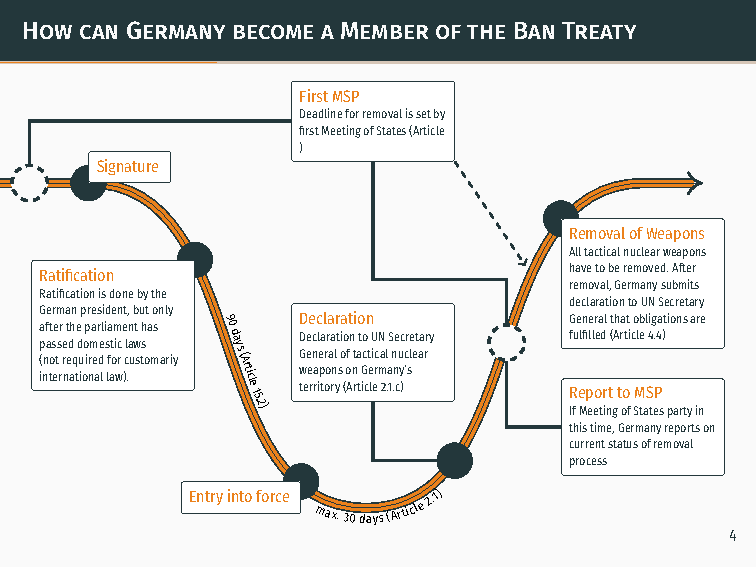
\includegraphics[width=\textwidth]{process}
\end{tcolorbox}
\end{column}



\begin{column}{0.3\columnwidth}
\tcbset{enhanced, colback=white, sharpish corners, fuzzy halo=0.5mm with fg,size=small,boxrule=0pt, height=0.75\textwidth}
\begin{tcolorbox}
\centering

\scriptsize
     Verification Options\\[0.8em]
 \tinyscriptsize
     We Trust You!\\[0.2em]
     Monitor Transport\\[0.2em]
     Declared Locations\\[0.2em]
     All-out Verification\\[0.2em]
\end{tcolorbox}
\end{column}
\end{columns}

\pause
\vspace{0.5cm}

\begin{block}{Final Thoughts}
Joining the Ban Treaty is possible for Germany

Implications can be promising, should be studied further

Verification is not required, but options exist
\end{block}

\begin{block}{Recommendations for Activists/Lobbyists}
Advocate jointly for removal and joining of ban treaty

Work jointly with other nuclear sharing states
\end{block}

\note{Notes
Tactical nuclear weapons are useless

Joining the ban would be relatively easy

Verification remains an open question}
\end{frame}



\appendix
\begin{frame}[label={sec:org0da5b12}]{Image References}
\tiny 

\textcolor{gray}{In order of appearance, own work not listed}\\[0.5em]

MGM-52C Lance: Public Domain, U.S. Army, \url{https://commons.wikimedia.org/wiki/File:MGM-52_Lance_02.jpg} (visited: 2018-03-09).\\[0.3em]

MGM-29 Sergeant: Public Domain, U.S. Army, \url{https://de.wikipedia.org/wiki/Datei:MGM-29_Sergeant_05.jpg} (visited: 2018-03-09).\\[0.3em]

Pershing 1 in West Germany: Public Domain, U.S. Army, \url{https://commons.wikimedia.org/wiki/File:OR_10.596B_13.png} (visited: 2018-03-09).\\[0.3em]
   
Medium Atomic Demolition Munition: Public Domain, Department of Defense, \url{https://de.wikipedia.org/wiki/Datei:Medium_Atomic_Demolition_Munition_(with_scientists).jpg} (visited: 2018-03-09).\\[0.3em]

W33 nuclear artillery projectile: Public Domain, U.S. Department of Energy, \url{https://en.wikipedia.org/wiki/File:Mk33.jpg} (visited: 2018-03-09).\\[0.3em]

Model of the W48 155-millimeter nuclear artillery shell: Public Domain, U.S. Department of Energy, \url{https://en.wikipedia.org/wiki/File:W48_155-millimeter_nuclear_shell.jpg} (visited: 2018-03-09).\\[0.3em]

MGR-1 Honest John in Hawaii: Public Domain, U.S. Army, \url{https://commons.wikimedia.org/wiki/File:MGR-1_Honest_John_06.jpg} (visited: 2018-03-09).\\[0.3em]

Nike-Hercules missiles in Section A of unit 1./FlaRakBtl 22: CC-BY 3.0, August Freimuth, \url{https://de.wikipedia.org/wiki/Datei:Nike_Hercules,_Sect._A,_Oedingen,_1980.JPG} (visited: 2018-03-04).\\[0.3em]

"A frontal view of four B-61 nuclear free-fall bombs on a bomb cart. (Released to Public) Location: BARKSDALE AIR FORCE BASE, LOUISIANA (LA) UNITED STATES OF AMERICA (USA) DoD photo by: SSGT PHIL SCHMITTEN Date Shot: 1 Dec 1986". B-61 bombs (probably trainers).: Public Domain, United States Department of Defense (SSGT Phil Schmitten), \url{http://de.wikipedia.org/wiki/Datei:B-61_bomb_rack.jpg} (visited: 2014-08-22).\\[0.3em]
\end{frame}

\begin{frame}[label={sec:org484ac85}]{Image References 2}
\tiny

Pershing II (MGM-31B): Public Domain, U.S. Army, \url{https://upload.wikimedia.org/wikipedia/commons/thumb/3/36/Pershing2MAN.jpg/797px-Pershing2MAN.jpg} (visited: 2018-03-09).\\[0.3em]

Fliegerhorst Büchel: CC-BY-SA 3.0, Stahlkocher, \url{http://commons.wikimedia.org/wiki/File:Büchel_Fliegerhorst.jpg} (visited: 2014-09-01).\\[0.3em]

German Tornado Refuelled by KC-10: Public Domain, U.S. Air Force photo/Staff Sgt. R. Alex Durbin, \url{https://commons.wikimedia.org/wiki/File:German_Tornado_refuelled_by_KC-10.jpg} (visited: 2018-03-09).\\[0.3em]

German Eurofighter during takeoff: CC-BY-SA 3.0, Krasimir Grozev / WIkimedia Commons, \url{https://de.wikipedia.org/wiki/Datei:German_eurofighter.JPG} (visited: 2018-03-10).\\[0.3em]

U.S. Air Force F-35A Lightning II Joint Strike Fighter: Public Domain, U.S. Air Force photo by Master Sgt. Donald R. Allen, \url{https://commons.wikimedia.org/wiki/File:F-35A_flight_(cropped).jpg} (visited: 2018-03-13).\\[0.3em]

Guido Westerwelle: CC-BY 3.0, Dirk Vorderstraße, \url{https://de.wikipedia.org/wiki/Datei:Westerwelle_hamm_2009.jpg} (visited: 2018-03-10).\\[0.3em]

Sigmar Gabriel: CC-BY-SA 3.0, Olaf Kosinsky / kosinsky.eu, \url{https://commons.wikimedia.org/wiki/File:2017-03-19_Sigmar_Gabriel_SPD_Parteitag_by_Olaf_Kosinsky-3.jpg} (visited: 2018-03-10).\\[0.3em]

Heiko Maas: CC-BY-SA 3.0, Sandro Halank, Wikimedia Commons, \url{https://commons.wikimedia.org/wiki/File:2017-03-26_Heiko_Maas_by_Sandro_Halank–1.jpg} (visited: 2018-03-10).\\[0.3em]
\end{frame}
\end{document}